The measurement of $H\rightarrow WW^*\rightarrow \ell\nu\ell\nu$ cross-sections relies on the accurate determination of a number of ``physics objects" within the detector primarily jets, missing transverse energy ($E_T^{miss}$), electrons, and muons. The final state particles of this interaction consist of one electron, one muon, and two neutrinos, which appear as missing transverse energy in the detector since they cannot be directly detected. The different flavored leptons are required in our final state to eliminate large contamination from Drell-Yan ($Z/\gamma^*\rightarrow ee/\mu\mu$) backgrounds. Drell-Yan backgrounds still play a role in our diferent flavor selection analysis but primarily come from far less numerous $Z/\gamma\rightarrow\tau\tau$ events which then decay to an electron and muon. Because our search focuses on VBF production Higgs, we also require two jets in the final state. Each physics object has a dedicated performance group which is tasked with providing recomendations for reconstruction, identification, isolation and measurements of efficiency, scale, and resolultion. Biasses or omissions in any of these would severely impact the precision of our analysis.Understanding the uncertainties associated with each reconstructed object is critical. In this chapter I briefly outline the algorithms used for tracking and isolation to accurately determine the kinematics of electrons, muons, jets and missing transverse energy. Particular attention will be paid to muons, as I spent a significant amount of time working in the Muon Performance Group applying and validating corrections to muon momentum scale and resolution. 

\section{Tracking}
Track reconstruction is fundamental to accurately identifying and describing electrons, muons and jets and primarily utilizes information from the ID. Charged particles entering the ID and solenoid field follow a circular trajectory in the transverse plane. They can be fully explained with a set of five parameters:
\begin{itemize}
\item $q/p_T$, the charged curvature where $q$ is electric charge and $p_T$ transverse momentum
\item $\phi$, the azimuthal angle
\item $\theta$, the polar angle
\item $d_0$, the transverse impact parameter or distance of closest approach of the beamspot position in the $x-y$ plane
\item $z_0$, the longitudinal impact parameter, or $z$ coordinate of the track at the point of closest approach. 
\end{itemize}
Track reconstruction calculates these decriptive parameters for each located track through an initial \textit{inside-out} procedure and second \textit{outside-in} method \cite{tracking}. First, track seeds are built from three hits in the silicon detectors, required to be in different silicon detector layers. Hits are then added to seeds moving away from the interaction point. If the final number of hits exceeds a determined threshold a track candidate is created and if not, the hits are discarded. Next for the \textit{outside-in} approach, segments are reconstructed in the TRT and silicon hits are added  through back-tracking. These is meant to find tracks from secondary interactions which don't begin at the primary interaction point. Requirements on hits, holes (points where measurement is expected but not found), and outliers (hits that reduce track fit quality) reduce probability of tracks which can not be matched to the primary vertex or secondary particules. The ATLAS Tracking Performance group determines reconstruction performance for tracks and demonstrate their robustness to potential fake track candidates and increased pile-up. Reconstructed tracks are used as input for the identification and measurement of kinematic variables for each of the physics objects that are decribed next in this chapter. 

In the ID, a pattern recognition algorithm reconstructs particle tracks with an inside-out sequence \cite{patternrecognition}. A track from a particle traversing the barrel typically has 3 pixel clusters, 8 SCT clusters and more than 30 TRT straw hits. The sequence begins by finding three-dimensional space points from the silicon hits. Each set of three space points which originate in the  interaction point are used to trace hits up to the outer edge of the silicon detector. The final track parameters are fit through a collection of hits that extend to the TRT \cite{IDreconstruction}.

\section{Electrons}
Accurate reconstruction and calibration of electrons within the ATLAS detector is integral to precision measurements, including the $H\rightarrow WW$ measurements in which an electron is required in the final state. Reconstruction, identification, and energy measurements of electrons and photons are the goals of the Electron and Photon Performance group.  This section will summarize each of these calibration processes and their performances with a focus on electrons. 

Electrons are defined through energy deposits in the calorimeter, the superclusters, each with a matching track from the ID. Photons are defined strictly through a calorimeter cluster.Figure \ref{figElectroReco} shows the procedure for electron and photon reconstruction. First, topo-clusters in the EM calorimeter and tracks in the ID are selected and matched together. Topo-clusters are defined based on signal to noise significance in calorimeter cells and calorimeter cell proximity. Standard reconstruction takes place in the ID and potential tracks are assigned to topo-clusters if their positions are within a region-of-interest compatible with that topo-clusters EM shower. Next, super-clusters are built from track-matched topo-clusters. Topo-clusters are tested for use as seed cluster candidates which begin super-clusters. Remaining topo-clusters are tested for compatibility as satellite clusters to each seed candidate. The resultant combination of seed and satellite clusters form super-clusters which are defined independetly for photons and electrons.  Finally, tracks are added to super-clusters, energy calibration and position corrections are applied, and analysis-level electrons and photons are created. Reconstruction efficiency for electrons is quite high, approaching the tracking efficiencyat high $p_T$. Photon reconstruction efficiency is significantly lower due to their dependence solely on calorimeter clusters \cite{ElectronPhotonPerformance}. 

\begin{figure}[!h]
        \centering
    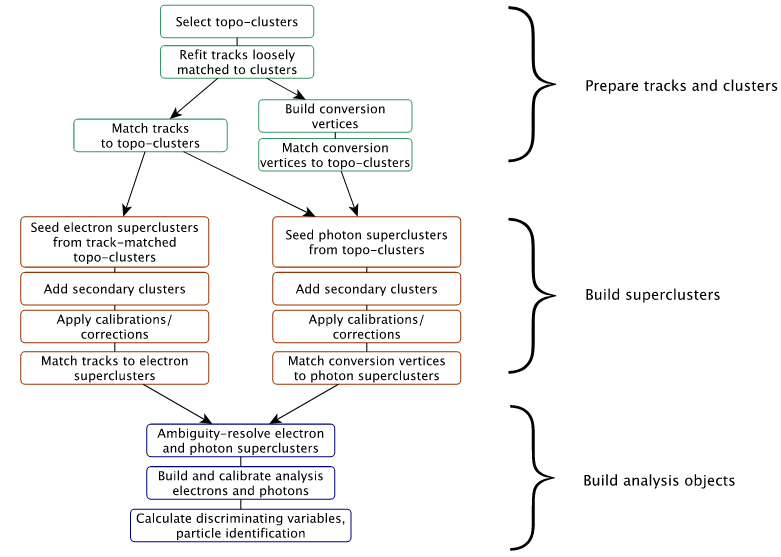
\includegraphics[width=.6\textwidth]{Pictures/ElectroReco.png}
    \caption{ Electron and photon reconstruction algorithm \cite{ElectronPhotonPerformance}}
    \label{fig:ElectroReco}
\end{figure}
 
Electron and photon energy resolution is determined from EM calorimeter showers and is optimized with multivariate regression algorithms. Energy scale is also corrected using calibration from $Z\rightarrow ee$ decays and verified with other $Z$-boson decays. Similarly, these calibrations are calculated for photons using $Z\rightarrow \ell\ell\gamma$. Systematic uncertainties that effect these calibrations include passive material between the interaction point and the EM calorimeter and pile-up \cite{ElectronPhotonPerformance}. 

While electron and photon objects are already identified and reconstructed, further `identification' selections are used to improve electron and photon purity. Prompt electrons are identified with a likelihood discriminant which takes into account track parameters and electromagnetic shower properties. The primary electron track must stretch into the two inner pixel layers and hit multiple points in the silicon-strip detector. The likelihood discriminant is calculated from probability density functions formed by smoothing histograms of 13 discriminating variables with an adaptive kernel density estimator.  These are calculated separately for both the likelihood that an event reconstructs a prompt electron (signal) or that it does not (background). These likelihoods are derived from $Z\rightarrow ee$ and $J/\Psi\rightarrow ee$ events recorded in Run-2. A tag-and-probe method is used to evaluate this likelihood - one electron in each decay must satisfy strict Run-1 likelihood discriminant requirements while the other serves as a probe of the new likelihood dscriminant. Three electron working points are derived- Loose, Medium, and Tight, each with lower efficiencies and higher purity than the previous. Physics analyses use the working points optimized for their analysis. For the $H\rightarrow WW$ measurement we use `Medium' reconstructed electrons. Figure \ref{fig:ElectronEff} shows electron identification efficiency for each of the working points in a sample of $Z\rightarrow ee$ events where efficiency is calculated through comparisons to MC simulated $Z\rightarrow ee$ and $J/\Psi\rightarrow ee$ events. The average efficiencies for electroweak processes are 93\%, 88\% and 80\%, respectively, for the Loose, Medium, and Tight operating points and gradually increase at high $E_T$ \cite{ElectronPhotonPerformance}.

\begin{figure}[!h]
        \centering
    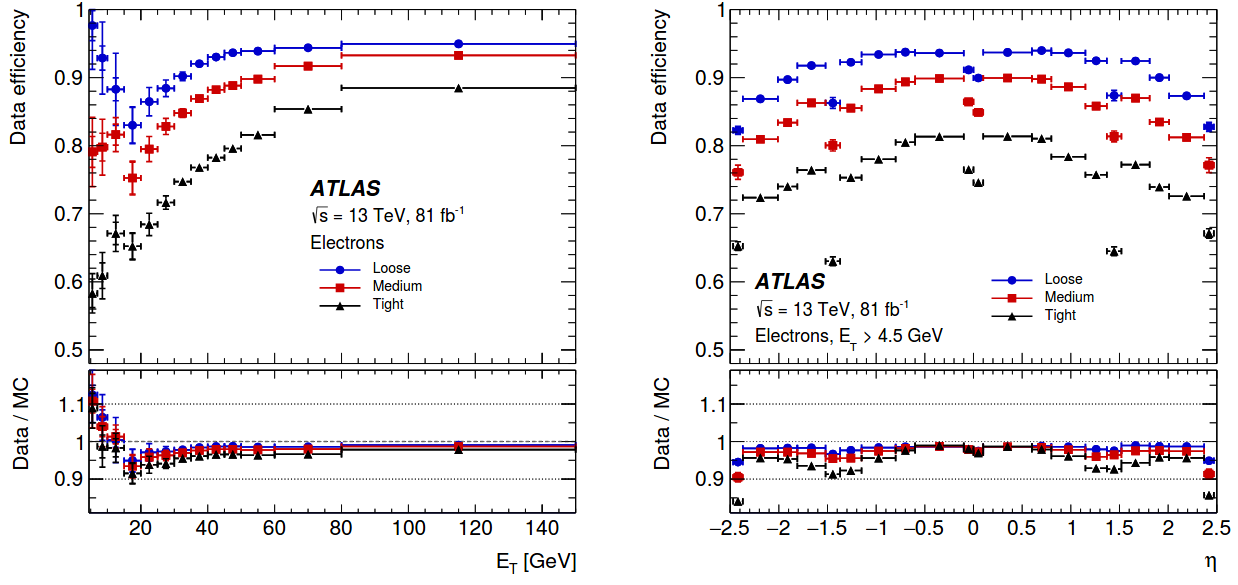
\includegraphics[width=.75\textwidth]{Pictures/ElectroEff.png}
    \caption{ Electron reconstruction efficiency as a function of $E_T$ (left) and $\eta$ (right) in $Z\rightarrow ee$ events for Losse, Medium, and Tight electrons \cite{ElectronPhotonPerformance}}
    \label{fig:ElectronEff}
\end{figure}

Track hits and calorimeter deposits near reconstructed electrons and muons can bias energy, momentum, and position measurements. Isolation performance is defined for calorimeter clusters by $E_T^{cone}$, the sum of transverse energy within a cone $\Delta R$ near a photon or electron cluster after correcting for leakage and pile-up effects. Track isolation $p_T^{cone}$ is defined as a sum of the transverse momentum of tracks within a cone about the electron track or interpolated photon track. For electrons the distance between nearby decay products is directly related to electron $p_T$ so a variable cone size can used such that 
\begin{equation}
\Delta R = \text{min}(\frac{10}{p_T},\Delta R_{max}),
\end{equation}
where $\Delta R_{max}$ is typically 0.2. Isolation working points strike a balance between efficiency and rejection of misidentified prompt electrons. The gradient working point is used by the $H\rightarrow WW$ analysis and gives an efficiency of 90\% at $p_T = 25$GeV and 99\% at $p_T = 60$GeV. These values are reached through cuts on $E_T^{cone20}$ and $p_T^{varcone20}$ derived from $J\Psi\rightarrow ee$ and $Z\rightarrow ee$ MC simulations. Isolation efficiency for electrons are shown in Figure \ref{fig:ElectronIsoEff} for Medium identified electrons in $Z\rightarrow ee$ events. The Gradient working point delivers efficiency that is stable across $\eta$ and is coupled with high background rejection of misidentified electrons \cite{ElectronPhotonPerformance}.  

\begin{figure}[!h]
        \centering
    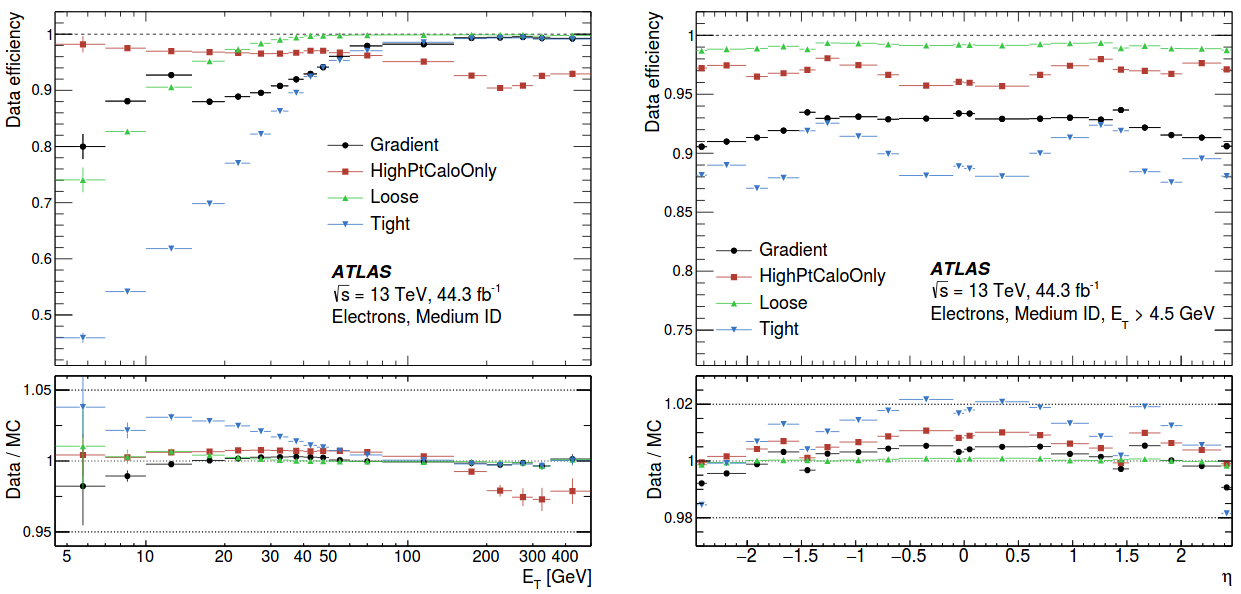
\includegraphics[width=.65\textwidth]{Pictures/ElectronIsoEff.png}
    \caption{ Electron isolation effiency shown for four working points in $Z\rightarrow ee$ events as a function of $E_T$ and $\eta$ \cite{ElectronPhotonPerformance}}
    \label{fig:ElectronIsoEff}
\end{figure}

Photon isolation is solely calorimeter-based. $Z\rightarrow \ell\ell\gamma$ events are used for photon isolation efficiency measurements and three working points are available which balance efficiency and background rejection just as in the electron case. 

Electron reconstruction, calibration, identification, and isolation are all integral for the $H\rightarrow WW$ analysis in order to accurately identify electrons in the final state of candidate Higgs events. Systematic uncertainties from electron identification and isolation efficiency will be discussed further in later chapters and play a significant role in $H\rightarrow WW$ cross-section measurements. 

\section{Muons}
Muons help lead to some of the most interesting physics analyses produced by the ATLAS experiment including $H\rightarrow WW\rightarrow \ell\nu\ell\nu$ measurements, which require a muon in the final state. The Muon Combined Performance group (MCP) is tasked with producing the most accurate muon calibrations for physics analyses. This includes defining muon identification and isolation criteria and measuring efficiency as well as muon momentum scales and resolutions. The group's goal is to create a number of ``working points'' tailored to different types of physics analyses. The working points are continuously updated and improved before being tested and implemented on different analyses. My work with the MCP group has focused on applying corrections necessary for muon momentum scale at the per mille level and resolution at the percent level in simulation to match the data. 

Muon reconstruction is performed independently using tracks reconstructed in the ID and MS and for combined tracks. This section will focus on reconstruction in the MS, which is particular to muons and the combined reconstruction, which uses information from both the ID and MS. 

Muon reconstruction begins with a search for hit patterns in each MS subdetector, which are called segments. The middle of the MS typically exhibits the largest number of trigger hits, therefore tracks are built by working out from the center of the MS and connecting segments layer-by-layer. Criteria such as hit multiplicity and fit quality determine track acceptance. At least two segments are needed to build a track. Hits associated with each track candidate are fitted using a global $\chi^2$ fit. A track candidate is accepted if it passes the selection criteria \cite{IDreconstruction}. 

The combined ID-MS reconstruction uses different algorithms to find different \textit{muon types}. There are four main types outlined below. When the same muon is reconstructed in more than one category, preference is given to Combined (CB), then Segment-tagged (ST), and finally Calorimeter Tagged (CT) muons. These algorithms have been continuously improved to increase precision, speed, and robustness against misidentification \cite{MCPpaper}.  

\begin{itemize}
\item \textbf{Combined muons (CB)}: They combine tracks from the ID and MS detectors using a global refit on all hits (some may be removed or added to improve quality). Most muons are reconstructed using an outside-in method. 
\item \textbf{Segment-tagged muons (ST)}: ST muons are assigned an ID track that is associated with at least one local MDT or CSC track after extrapolation. These are used when muons cross only one layer of the MS because of low $p_T$ or regions out of most MS layer boundaries. 
\item \textbf{Calorimeter-tagged muons (CT)}: These muons are identified by an ID track that can be matched to a minimum ionizing particle energy deposit in the calorimeter. They have the lowest purity but are optimized for $|\eta|  < 0.1$ and $1.5 < p_T < 100$ GeV where the MS is only partially instrumented. 
\item \textbf{Extrapolated muons (ME)}: They are reconstructed in the MS with the addition of silicon points and with a loose requirement that the muon track originated at the IP. In general, these muons are required to traverse $2-3$ layers of MS chambers. These are mainly used to extend acceptance in the region $2.5 < |\eta| < 2.7$, which is not covered by the ID. 
\end{itemize}

In order to distinguish muons from other particles (like backgrounds from pion and kaon decays) strict quality requirements must be set to select prompt muons with high efficiency. Reconstruction targets $W$ and $Z$ decays (as opposed to light-hadron decays) which originate from the interaction point. We use the following variables to identify such muons:
\begin{itemize}
\item \textit{q/p significance}, the absolute value of the difference between the ratio of the charge and momentum of muons in the ID and MS divided by the sum in quadrature of their corresponding uncertainties
\item \textit{$\rho^\prime$}, the absolute value of the difference between the $p_T$ measurements in the ID and MS divided by the $p_T$ of the combined track 
\item \textit{$\chi ^2$}, the normalized fit parameter of the combined track
\end{itemize}

Specific requirements on the number of hits in the ID and MS assure that inefficiencies are expected and momentum measurements are robust. There are four muon identification selections that each addresses specific needs of physics analyses \cite{MCPpaper}.

\begin{itemize}
\item \textbf{\textit{Loose} Muons}: The \textit{Loose} criteria maximizes the reconstruction efficiency, losing very few potential muons, while providing satisfactory tracks. All muon types are used in this criteria.
\item \textbf{\textit{Medium} Muons}: \textit{Medium} is the default selection for muons in ATLAS because it minimizes systematic uncertainties associated with reconstruction and calibration. Only CB and ME tracks are used with requirements for over 3 hits in at least two MDT layers in most regions. All \textit{Medium} muons are included in the \textit{Loose} criteria.
\item \textbf{\textit{Tight} Muons}: \textit{Tight} selects muons with the highest purity, but sacrifices efficiency. All \textit{Tight} muons are included in the \textit{Medium} selection, but only CB muons with at least two hits in the MS are considered, and the $\chi^2$ value must be less than $8$.  
\item \textbf{\textit{High-$p_T$} Muons}: \textit{High-$p_T$} muons have good momentum resolution for tracks with $p_T > 100$ GeV. This is beneficial to searches for high-mass $Z^\prime$ and $W^\prime$ resonances. CB muons in the \textit{Medium} selection with at least $3$ hits in $3$ MS stations are included. 
\end{itemize}

The $H\rightarrow WW$ analysis uses Tight muons with the added condition that $p_T>15$ GeV and $\eta<2.5$ to gain the highest purity possible and eliminate background from misidentified leptons, which constitute a significant background even with this selection. 

We measure the muon reconstruction efficiency in two different ways in the regions $|\eta|  < 2.5$ and $2.5 < |\eta|  < 2.7$. First, in the barrel region, we use the \textbf{Tag-and-Probe} method. In this method we select an almost-pure sample of $J/\psi$ and $Z$ decays and require the leading muon to be a \textit{Medium} muon labeled the \textbf{tag}. The subleading muon, the \textbf{probe}, must be reconstructed independently. There are three types of probes:
\begin{itemize}
\item \textbf{ID track}: Allows measurement of MS efficiency and of tracks not accessible to CT muons. 
\item \textbf{CT tracks}: Allows measurement of MS efficiency and has powerful rejection of background (especially at low $p_T$). This is the most commonly used probe. 
\item \textbf{MS tracks}: Allows measurement of ID and CT efficiency.
\end{itemize}

To find the overall efficiency of \textit{Medium, Tight,} or \textit{High-$p_T$} muons, we multiply the efficiencies associated with each type of probe. The efficiency  $\epsilon$(X$|$CT) (X $=$ \textit{Medium / Tight / High-$p_T$}) of reconstructing these muons assuming a reconstructed ID track is measured using a CT muon as probe. This result is corrected by the efficiency $\epsilon$(ID$|$MS) of the ID track reconstruction measured using MS probes.
\begin{equation}
\epsilon \textrm{(X$|$ID)} \cdot \epsilon \textrm{(ID)} = \epsilon \textrm{(X$|$CT)} \cdot \epsilon \textrm{(ID$|$MS)} \hspace{20 pt} (\textrm{X} = Medium/Tight/High\textrm{-}p_T)
\end{equation}
The ID track reconstruction efficiency must be independent from the muon spectrometer track reconstruction ($\epsilon$(ID) $= \epsilon$(ID$|$MS)). In addition, the use of a CT muon as a probe instead of an ID track must not affect the probability for \textit{Medium, Tight,} or \textit{High-$p_T$} reconstruction ($\epsilon$(X$|$ID) $= \epsilon$(X$|$CT)). These assumptions are largely true with simulations showing some small deviations. These deviations are taken into account when calculating systematic errors. 

The reconstruction efficiency of \textit{Loose} muons is measured separately for CT muons within $|\eta| < 0.1$ and all other \textit{Loose} types. The CT muon efficiency is measured using MS probe tracks, and the efficiency of other muons is evaluated similarly to the \textit{Medium, Tight,} and \textit{High-$p_T$} muons using CT probe muons \cite{MCPpaper}. For $|\eta| > 2.5$, the efficiency is calculated using the ME muons in the \textbf{Loose} and \textbf{Medium} selections. The number of muons observed in this region is normalized to the number of muons observed in the region $2.2 < |\eta| < 2.5$. A more detailed discussion of the efficiency measurement in this region can be found in Ref \cite{oldMCPpaper}. 

\textbf{Scale factors} are defined as the ratios between the efficiency of data and the efficiency of Monte Carlo simulations. They are used to describe the deviation between simulated and real detector behavior and are used in physics analyses to correct simulations. 
\begin{figure}[!h]
  \centering
  \begin{minipage}[b]{0.45\textwidth}
    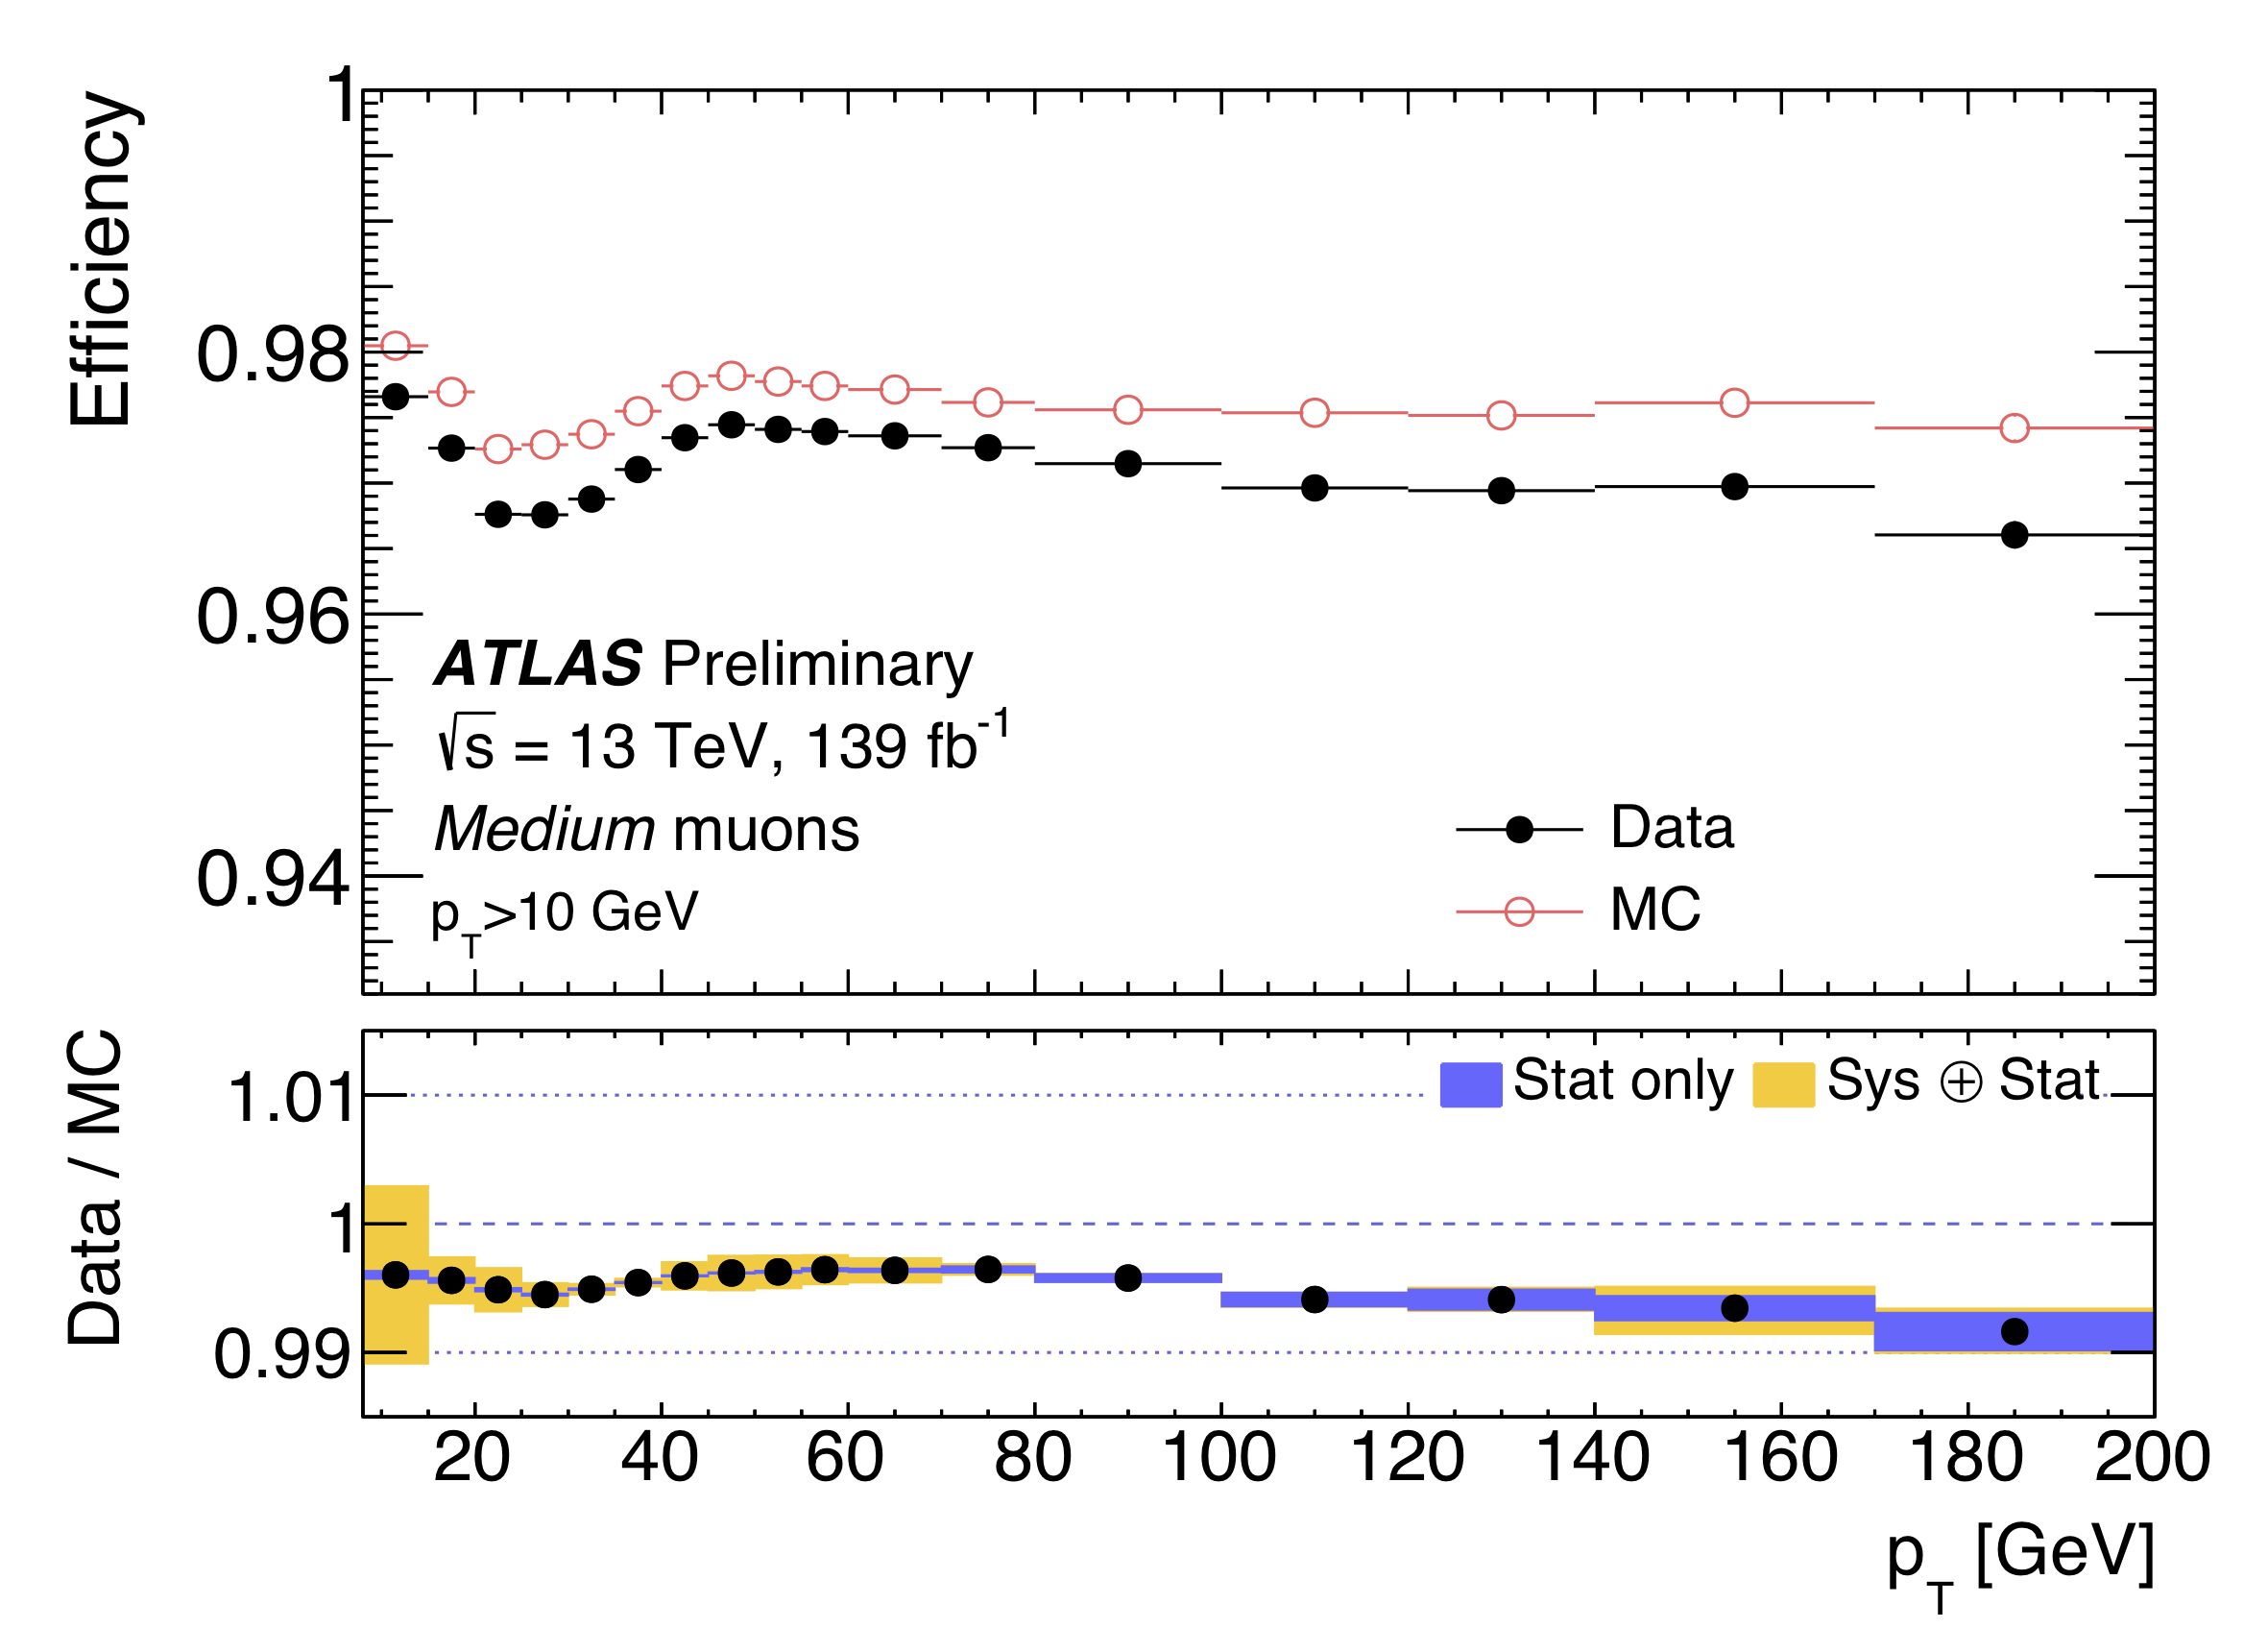
\includegraphics[width=\textwidth]{Pictures/efficiencyoverpt.PNG}
  \end{minipage}
  \hspace{.5cm}
  \begin{minipage}[b]{0.45\textwidth}
    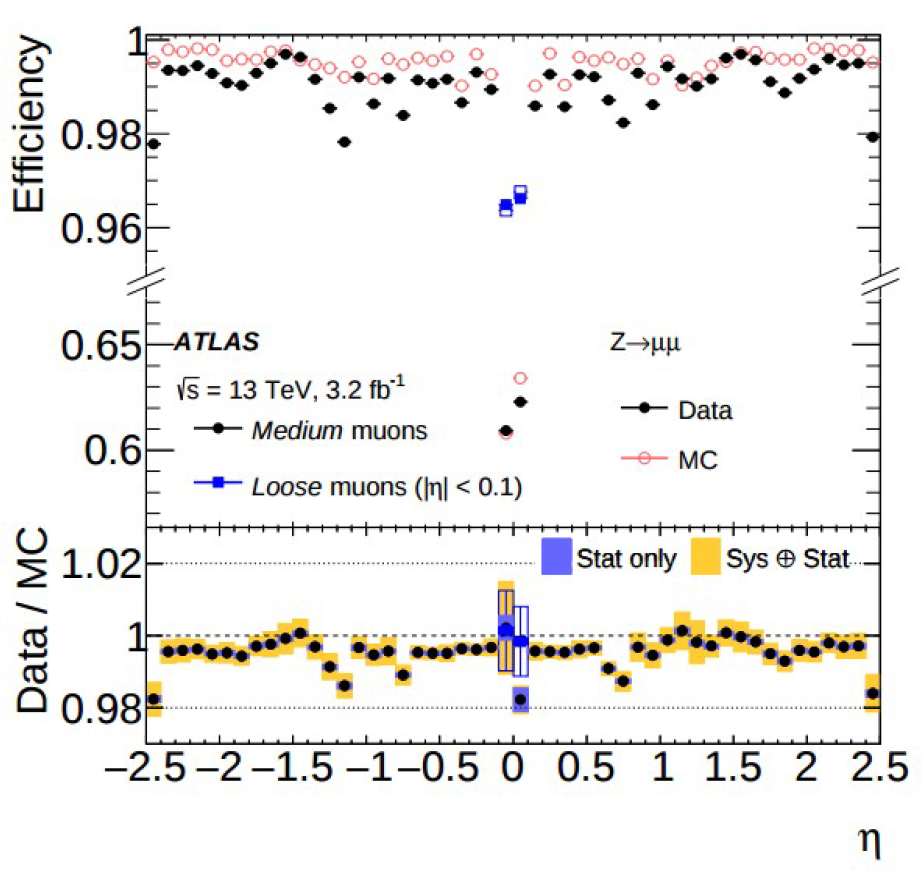
\includegraphics[width=\textwidth]{Pictures/efficiencyovereta.PNG}
  \end{minipage}
  \caption{On the left, reconstruction efficiency for \textit{Tight} muons from $Z \rightarrow \mu\mu$ events is displayed as a function of the $p_T$ of the muon in the region $0.1 < |\eta| < 2.5$ with systematic and statistical uncertainties.  On the right, muon reconstruction efficiency is shown as a function of $\eta$ in $Z \rightarrow \mu\mu$ events for muons with $p_T > 15$ GeV for \textit{Medium}, \textit{Loose} and \textit{Tight} muons. In both plots the full 139fb$^{-1}$ Run-2 dataset is used\cite{MCPPlots}.}
  \label{fig:efficiency}
\end{figure}

Figure \ref{fig:efficiency} displays reconstruction efficiency for \textit{Medium} muons over a range of $p_T$ and all other working plotted over $\eta$. While \textit{Medium} muons have a a higher efficiency than the \textit{Tight} selection used in this analysis, both have an efficiency above 95\% for a large range of $\eta$ and $p_T$. $J/\psi$ decays probe low $p_T$ muons while $Z$ decays probe muons of a higher $p_T$ allowing a large range to be defined. MC simulations match data within $1-2\%$. The only significant loss of efficiency is seen at extremely low $\eta$ due to criteria excluding ID muons. Overall, the default \textit{Tight} muon selection demonstrates reconstruction efficiency around $95\%$ for muons in our selection $p_T$ range.

Isolation distinguishes muons from $W$/$Z$ decays from those produced in the decay of $b$ and $c$ mesons. When heavy particles like $W$, $Z$, and Higgs bosons decay they often produce muons in isolation. Semileptonic decays of $b$ and $c$ hadrons, on the other hand, typically produce muons embedded in jets.

The MCP group uses two muon isolation variables: a track-based variable ($p_T^{varcone30}$) and a calorimeter-based variable ($E_T^{topocone20}$). $p_T^{varcone30}$ is defined as the scalar sum of the transverse momenta of tracks with $p_T > 1$ GeV in a cone around the muon of transverse momentum $p_T$ excluding the muon track itself. The cone size is $p_T$-dependent to improve the performance for muons produced in decays with a large transverse momentum. $E_T^{topocone20}$ is defined as the sum of the transverse energy of topological clusters in a cone around the muon after subtracting the contribution from the energy deposit of the muon itself and correcting for pile-up effects \cite{jets}. 

Table \ref{tab:datasetsdef} defines seven isolation selection criteria - called ``isolation working points'' - that optimize different physics analyses. The\textit{LooseTrackOnly} and \textit{FixedCutTightTrackOnly} working points are defined by cuts on the relative track-based isolation variable. All other working points are defined by cuts applied separately on both relative isolation variables. All cuts are tuned as a function of the $\eta$ and $p_T$ of the muon to obtain a uniform performance. The target efficiencies of the different working points are described in Table \ref{tab:isolation}. The efficiencies for the seven isolation working points are measured in data and simulation using the \textbf{Tag-and-Probe} method described previously. Figure \ref{fig:isolation} shows the isolation efficiency measured for \textit{Medium} muons in data and simulation as a function of the muon $p_T$ for two different working points. In both the \textit{GradientLoose} and \textit{FixedCutTightTrackOnly} working points, efficiency is above $90\%$ and matches simulation well within errors for muons for higher $p_T$ muons. In the $HWW$ analysis, fixed isolation cuts are optimized independent of Muon Performance working points. Only muons with $p_T>15$ GeV are considered so the efficiency is optimized for muons which pass this and the \textit{Tight} selection cuts.  

\begin{table}[!h]
	\centering 
    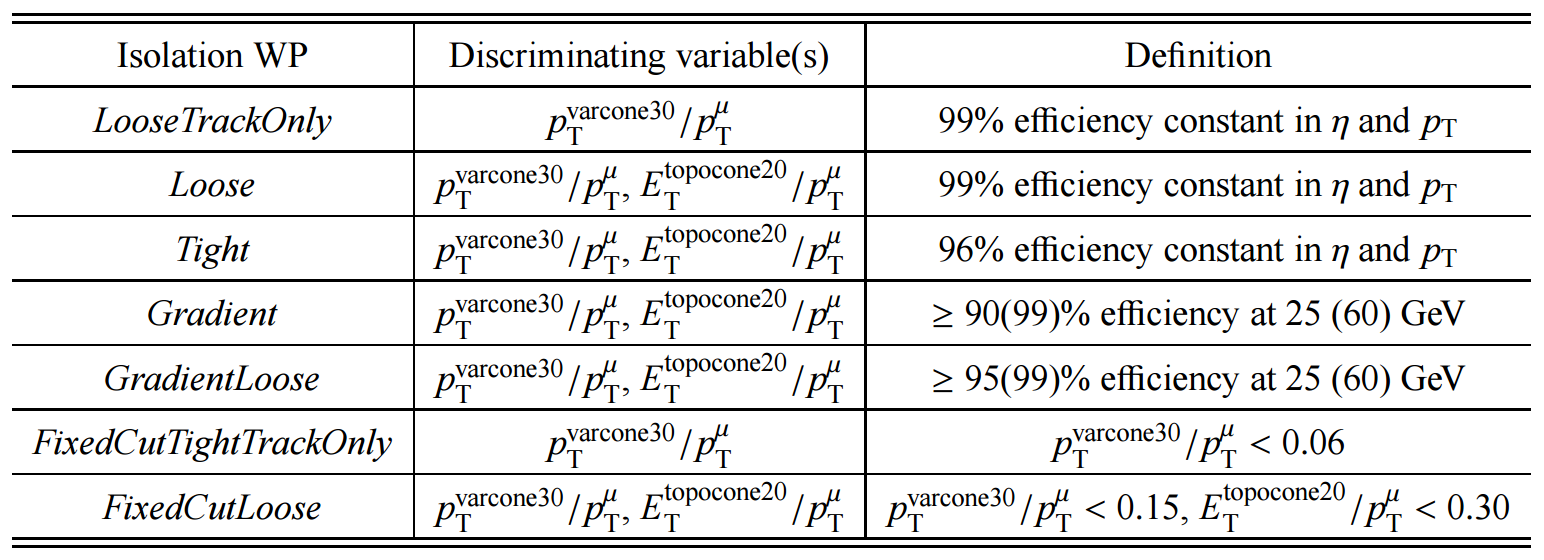
\includegraphics[width=.9\textwidth]{Pictures/isolationworkingpoints.PNG}
    \caption{The seven isolation working points are described by their discriminating variables and defining criteria \cite{MCPpaper}.}
    \label{tab:datasetsdef}
\end{table}

\begin{figure}[!h]
  \centering
  \begin{minipage}[b]{0.47\textwidth}
    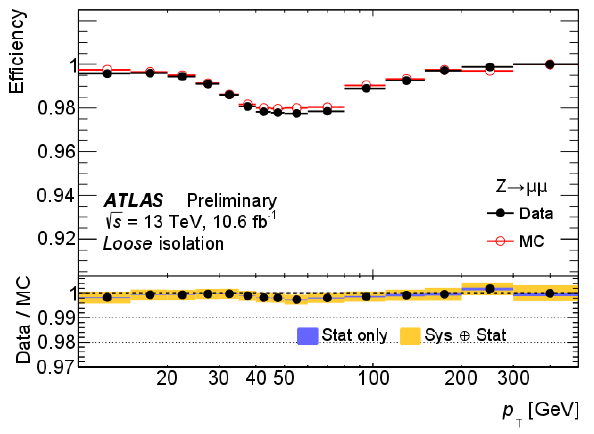
\includegraphics[width=\textwidth]{Pictures/isolationefficiency1.png}
  \end{minipage}
  \hspace{.2cm}
  \begin{minipage}[b]{0.48\textwidth}
    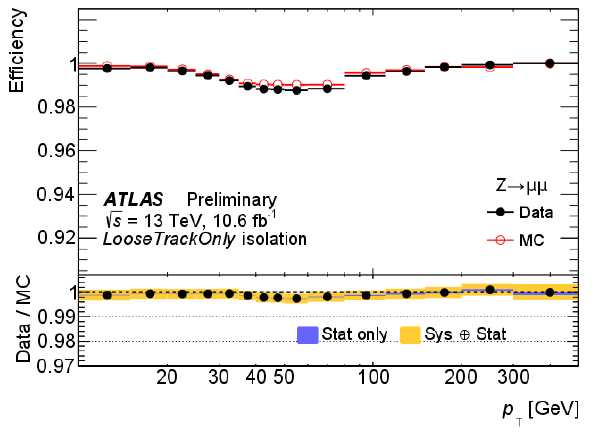
\includegraphics[width=\textwidth]{Pictures/isolationefficiency2.png}
  \end{minipage}
  \caption{Isolation efficiency for the GradientLoose (left) and FixedCutTrackOnly (right) muon isolation working points. The efficiency is displayed as a function of $p_T$ in $Z \rightarrow \mu\mu$ events. The black markers show efficiency measured in data samples while the red show MC simulations. The bottom panel shows the ratio of the efficiency between the two as well as both statistical and systematic uncertainties \cite{MCPPlots2}.}
  \label{fig:isolation}
\end{figure}

The isolation cuts used by the $H\rightarrow WW$ analysis are $p_T^{varcone30}/p_T<0.06$ and $p_T^{topocone20}/p_T<0.09$ which are relatively tight selections and designed to reduce misidentified lepton backgrounds. 

The muon momentum scale and resolution are studied using $Z$ and $J/\psi$ decays. In order to obtain agreement between simulation and data in muon momentum scale to the per mille level and in resolution to the percent level, we need to apply a set of corrections to the simulated muon momentum. After applying the corrections we validate them by comparing the muon momentum scale and resolution between simulation and data over $\eta$, $\phi$, and $p_T$.

We extract the calibration parameters with the transverse momentum of the ID and MS components of a CB track.  The corrected transverse momentum is described by the following equation: 

\begin{equation}
    p_T^{\textrm{Cor,Det}} = \frac{p_T^{\textrm{MC,Det}}+\sum\limits_{n=0}^1s_n^{\textrm{Det}}(\eta,\phi)(p_T^{\textrm{MC,Det}})^n}{1+\sum\limits_{m=0}^2\Delta r_m^{\textrm{Det}}(\eta,\phi)(p_T^{\textrm{MC,Det}})^{m-1}g_m} .
\end{equation}
Here the $g_m$ terms are normally distributed random variables with zero mean and unit width. The $\Delta r $ and $s$ terms describe momentum resolution smearing and scale corrections applied in specific detector regions, respectively. Both the ID and MS are divided into $18$ pseudorapidity regions and the MS is divided into two $\phi$ bins separating the large and small sectors. Each of these bins leverages different alignment techniques and has different material distributions. 

There are two $s$ terms that represent different types of corrections. $s_1$ corrects for inaccuracy in the description of the magnetic field integral and the detector in the direction perpendicular to the magnetic field. $s_0$ corrects for the inaccuracy in the simulation of energy loss in the calorimeter and other materials. Since this loss is negligible in the ID, it is only nonzero in the MS \cite{MCPpaper}.

The denominator introduces momentum smearing which broadens the $p_T$ resolution in simulation. The parametrization of the smearing is defined as
\begin{equation}
    \frac{\sigma(p_T)}{p_T} = r_0/p_T \oplus r_1 \oplus r_2 \cdot p_T .
\end{equation}
In this equation $r_0$ is related to the fluctuations in energy loss in the traversed material, $r_1$ accounts for multiple scattering, local magnetic field inhomogeneities, and local radial displacements of hits, and $r_2$ describes intrinsic resolution effects caused by the spatial resolution of the hit measurements and by residual misalignment of the MS \cite{MCPpaper}. 
Correction parameters are extracted from data using a binned maximum-likelihood fit with templates derived from simulation which compares the invariant mass distributions for $J/\psi$ and $Z$ decay candidates in data and simulation. The muons are carefully selected to be compatible with tracks that start at the interaction point and penetrate both the ID and the MS. Muons are also selected to pass specific momentum and isolation criteria. The dimuon mass distribution of these tracks in data is fitted using a Crystal Ball function convoluted with an exponential background distribution in the ID and MS fits. The background model and its normalization are then used in the template fit. The fits are performed in $\eta-\phi$ regions of fit (ROFs) which compromise regions with uniform features in the ID and MS \cite{MCPpaper}. 

From these fits, we can find the smearing terms across all $\eta$ regions. Once the corrections are applied, we can validate that the agreement between data and MC is excellent. This is shown in Figure \ref{fig:parametrizationeta}. $r_0$ is set to zero across all $\eta$ regions since energy loss is negligible in the ID. $r_1$ and $r_2$ increase as $\eta$ increases since spatial resolution decreases and inhomogeneities increase as as we move from the barrel to end-cap regions of both the ID and MS. Muon momentum corrections are continuosly studied during ATLAS runs to validate muon calibration performance and account for discrepancies.

\begin{figure}[!h]
	\centering 
    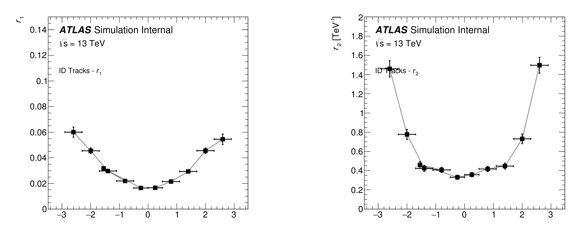
\includegraphics[width=.85\textwidth]{Pictures/parametrizationIDeta.PNG}
    \caption{ The $r$- values from each of $10$ fits of resolution to $p_T$ for ID muon simulations are shown. Each value corresponds to a particular ROF or $\eta$ region. These plots show $r_1$ (left) and $r_2$  (right) as functions of leading muon $\eta$.}
    \label{fig:parametrizationeta}
\end{figure}

\section{Jets}
Quarks and gluons emitted from high-energy hard scattering do not appear in the detector directly. Quarks and gluons with high enough energye radiate low energy gluons until partons are able to bind into color-neutral hadrons. These hadrons are collimated in groups as ``jets". Jet energy and momentum are used in physics analyses as proxies for initial scattered partons. Pile-up presents the main difficulty in jet calibration as multiple interactions occuring in the detector at once create significant, often hadronic, background. The hard interaction of interest must be separated from pile-up background, which is most often soft. During Run-1, the ATLAS experiment reconstructed jets using either only the calorimeter or the tracker, though most often the calorimeter. Topological clusters of calorimeter cells (topo-clusters) were used to trace jet tracks. At the end of Run-1, the jet energy scale (JES) correction factor used to calibrate jets to the particle level was re-calculated using additional track information from the Inner Detector and Muon Spectrometer, which greatly improved jet resolution \cite{JetRun1}. 

In Run-2, a new algorithm for jet reconstruction took advantage of the improvements shown in Run-1 by including information from the tracker. `Particle flow' uses the tracker's higher momentum resolution for low-energy charged particles and its greater angular resolution of single charged particles. This is complemented by the calorimeter's ability to reconstruct both charged and neutral particles and the calorimeter's higher energy resolution for high energy physics objects. The calorimeter also has an extended acceptance so in the forward region only calorimeter topo-clusters are used. One potential difficulty with the `particle flow' algorithm is the possibility for double counting particles if the jets reconstructed by the tracker are not properly matched with the corresponding calorimeter signals. This is avoided in the algorithm through the condition that if a particle's track measurement is used, its corresponding energy must be subtracted from the calorimeter measurement. The success of the algorithm in removing only energy deposits from the tracked jet represents a key criteria for its overall performance \cite{ParticleFlow}.

\begin{figure}[!h]
        \centering
    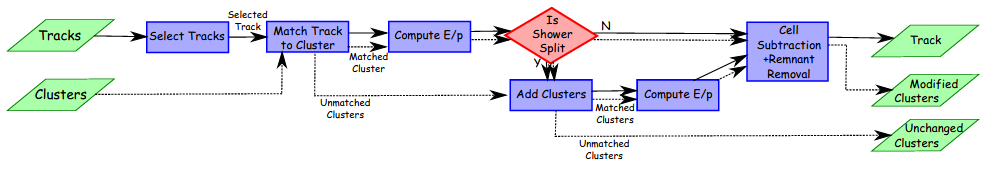
\includegraphics[width=.85\textwidth]{Pictures/ParticleFlow.png}
    \caption{Flow chart of the particle flow algorithm beginning with track selection and ending with charged particles and changed/unchanged topo-clusers \cite{ParticleFlow}.}
    \label{fig:ParticleFlow}
\end{figure}

Topo-clusters are described by two main properties - $\epsilon$, which represents the fraction of true energy deposited in the cluster out of the total true energy deposited in all topo-clusters for that object, and $\rho$, the fraction of a particle's true energy which lies within the topo-cluster. High $\rho$, high $\epsilon$ topo-clusters allow contributions from different particles to be distinguished and so are easier to apply hadronic shower subtraction \cite{ParticleFlow}.

Jet tracks need to meet strict criteria. In this analysis, tracks included in jets are required to satisfy the ``tight'' selection criteria, which includes requirements for at least nine hits in silicon detectors, no missing Pixel hits, $\eta<2.5$, and $40>p_T>0.5$ GeV. High $p_T$ tracks are excluded because of their poor isolation. In addition, tracks which are identified as electrons or muons are excluded \cite{ParticleFlow}. 

With topo-clusters and tracks assembled, the algorithm matches each to one another. Topo-clusters are ranked through the distance metric 
\begin{equation}
\Delta R' = \sqrt{(\frac{\Delta \phi}{\sigma_\phi})^2+(\frac{\Delta \eta}{\sigma_\eta})^2},
\end{equation}
where $\sigma_\phi$ and $\sigma_\eta$ denote angular topo-cluster widths. A requirement that $E^{clus}/p^{trk}>0.1$ is applied so that the energy of the topo-cluster must contain a significant portion of the energy of the track. This requirement rejects about $30-40\%$ of the incorrect topo-clusters at $p_T>5$ GeV. The closest topo-cluster to each track in $\Delta R'$ is taken to be the correct match. If no topo-cluster is within a cone of $\Delta R'= 1.64$ it is assumed that the particle did not form a topo-cluster in the calorimeter \cite{ParticleFlow}. 

Topo-clusters are thus matched to particle tracks and the energy deposited by the particle is subtracted from the calorimeter. The average energy deposited by a particle with momentum $p^{trk}$ is $<E_{dep}>=p^{trk}<E_{ref}^{clus}/p_{ref}^{trk}>$, where $<E_{ref}^{clus}/p_{ref}^{trk}>$ is calculated using single-particle samples without pile-up by summing topo-cluster energies within $\Delta R = 0.4$ about the track position. These are calculated at varying $p_T$ and $\eta$ values to capture effects from detector geometry and shower development. Particles often split their energy between multiple topo-clusters and this split can be determined through the significance of the difference between expected energy and that of the matched topo-cluster. This new full set of matched clusters is considered for energy subtraction \cite{ParticleFlow}. 

Energy subtraction is performed cell-by-cell unless $<E_{dep}>$ is greater than the energy of the total matched topo-clusters, in which case they are all removed. Rings are formed in ($\eta,\phi$) about the extrapolated track and are one calorimeter cell wide. The average energy density in each ring is computed and the ring with the highest energy density is subtracted first. This continues to lower density rings until $<E_{dep}>$ is reached. Finally, energy clusters from shower fluctuations are removed. Ideally now the sum of selected tracks and remaining topo-clusters together represent the reconstructed event without double counting. An example display of particle flow events is shown in Figure \ref{fig:ParticleFlowExample}

\begin{figure}[!h]
        \centering
    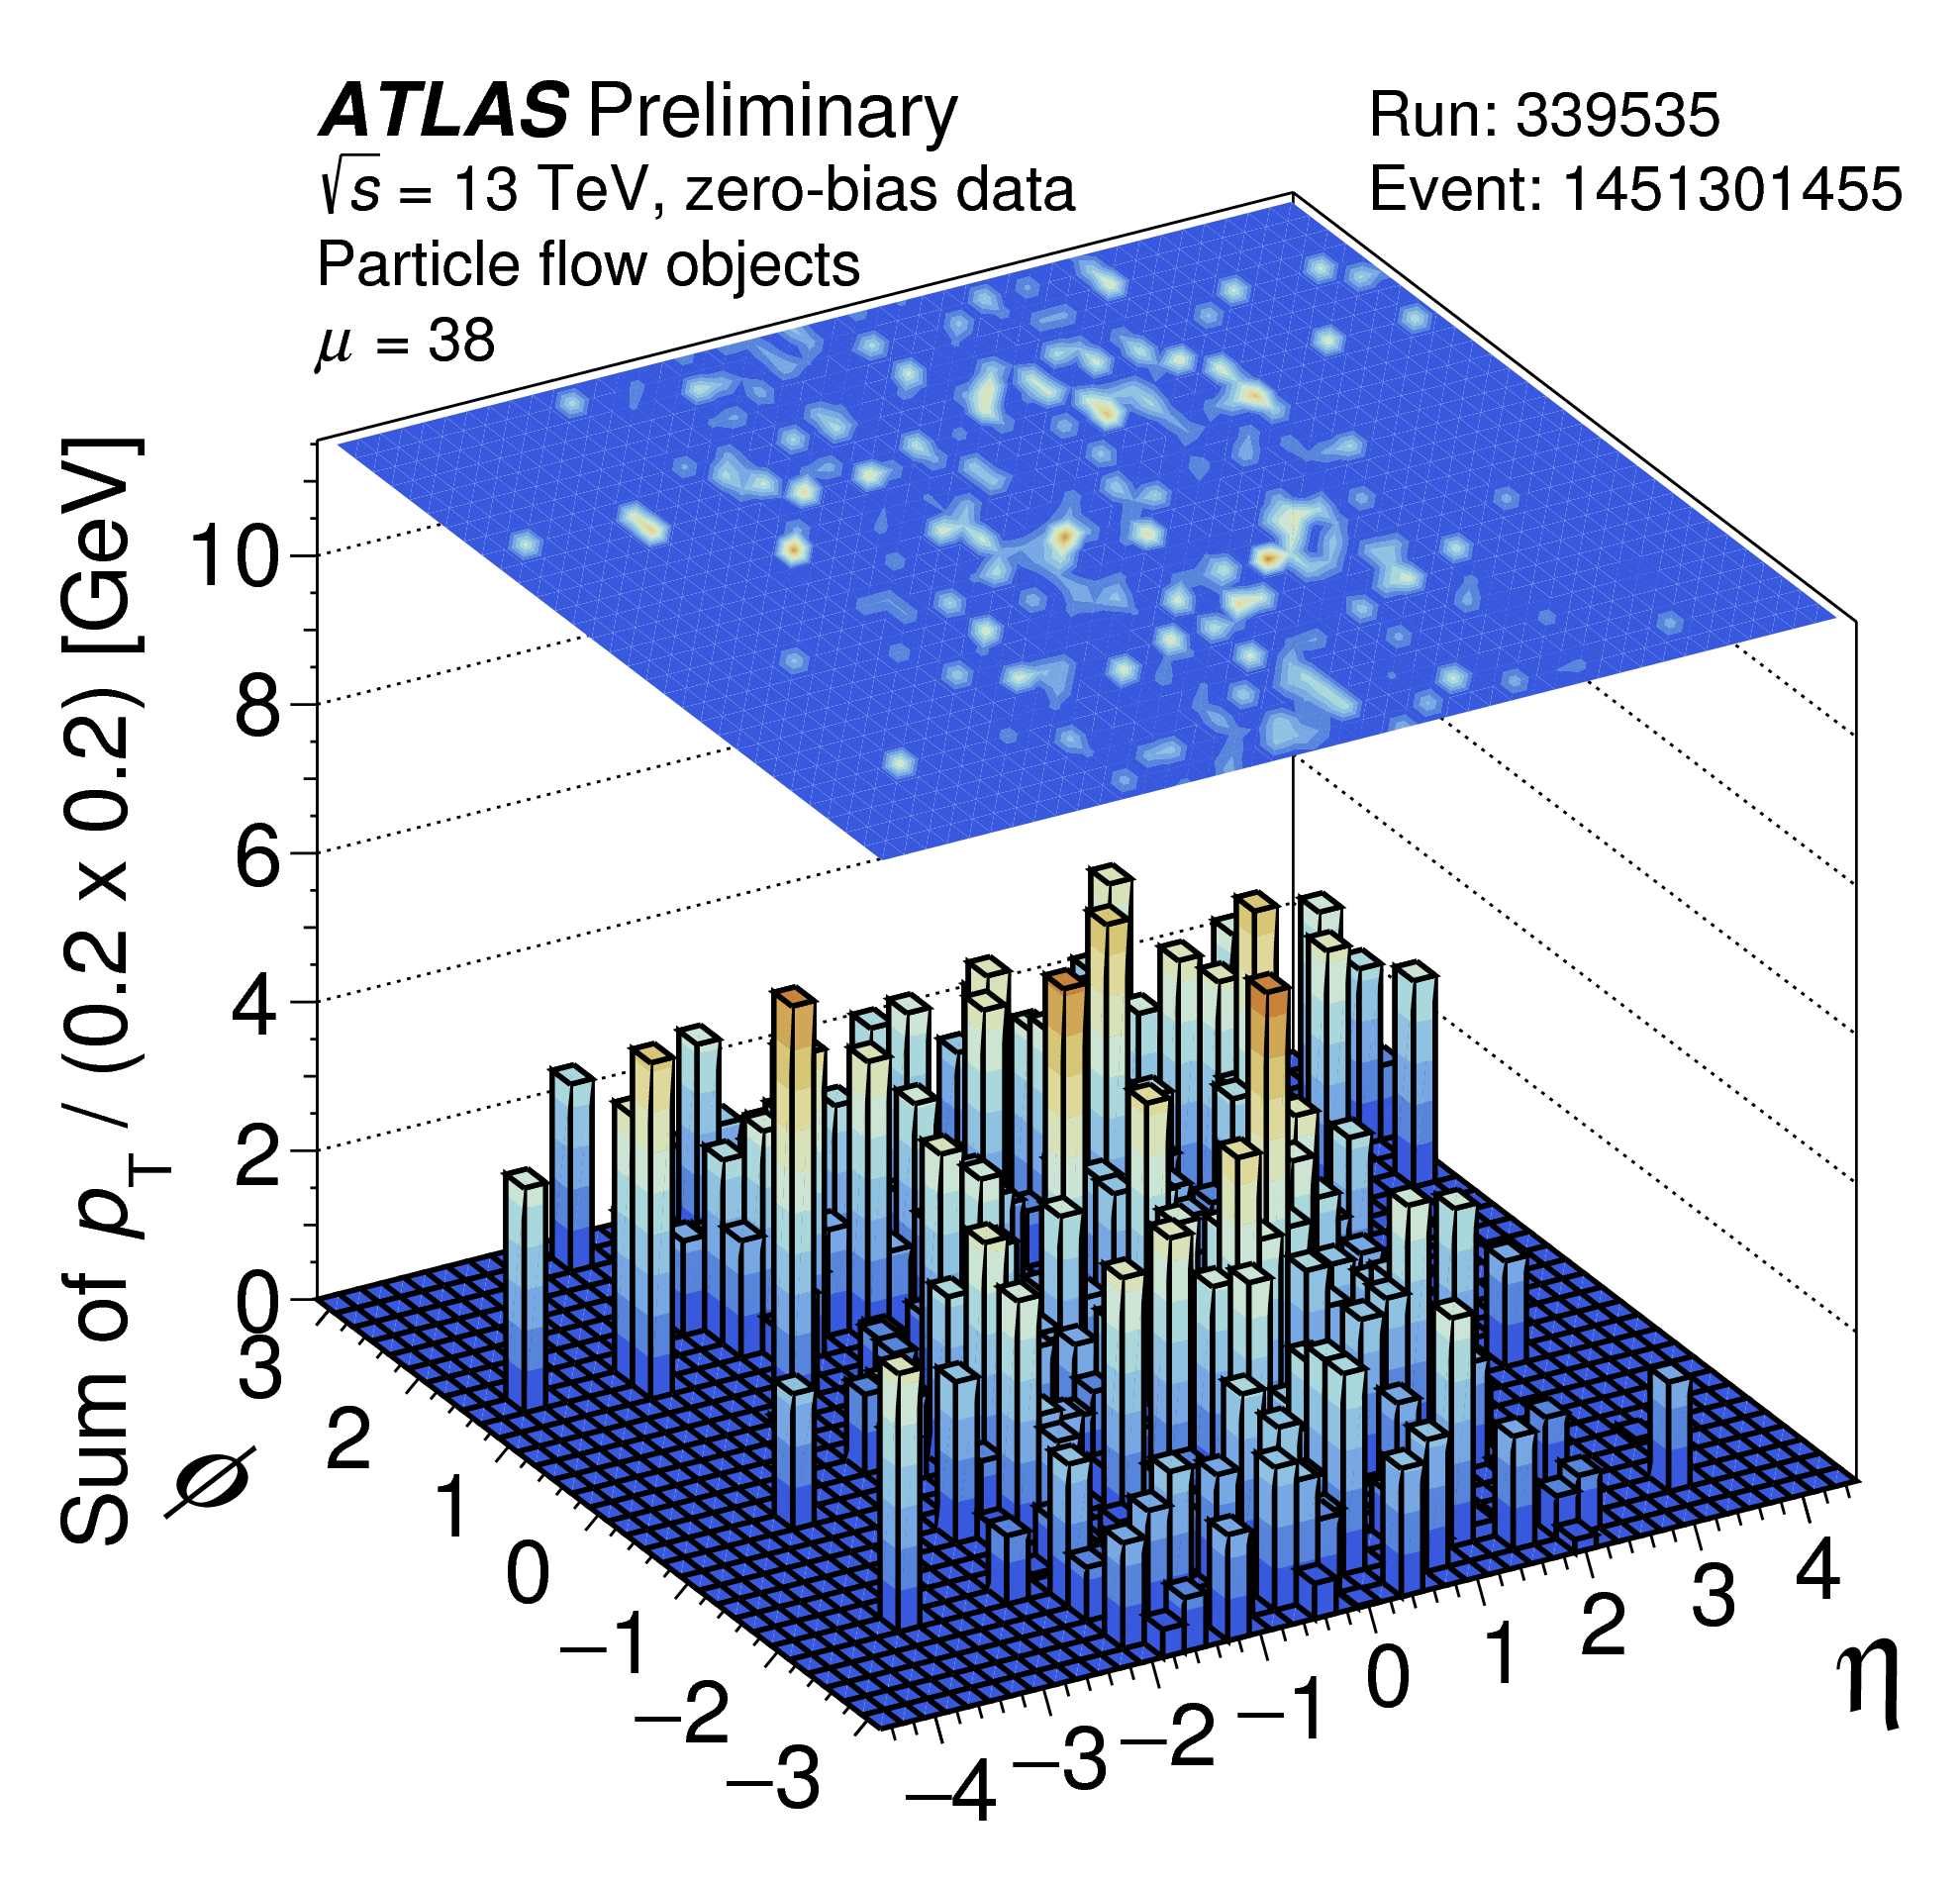
\includegraphics[width=.4\textwidth]{Pictures/ParticleFlowExample.png}
    \caption{Sum of transverse momenta of neutral and charged particle flow objects in an area $\Delta \eta \times \Delta\phi = 0.2 \times 0.2$ from a 2017 event with mean number of interactions per beam crossing $\mu=38$ \cite{JETEtmiss}}
    \label{fig:ParticleFlowExample}
\end{figure}

Jet-finding algorithms aim to approximate the hadrons that generate calorimeter and track-based jets in the detector. They bridge the divide between observable jet objects and theoretical predictions from QCD. There are several jet algorithms in use currently and all are collinear and infrared safe. This means that neither splitting a jet collinearly nor soft emissions should change jet structure. Without these properties perturbation theory diverges at high orders.

Anti-$k_t$ is the jet algorithm used by ATLAS and is infrared collinar-safe by construction and resilient to soft radiation \cite{antikt}.
%Distance between pseudojets $i$ and $j$, $d_{ij}$ and the distance between pseudojet $i$ and the beam $d_{iB}$ are defined. The algorithm loops through these distances beginning with the smallest distance. If $d_{ij}$ is smallest, pseudojets $i$ and $j$ are combined, if $d_{iB}$ is smallest then $i$ is a jet and removed from the list. This continues iteratively until all jets are defined. The distances are defined:
%\begin{equation}
%\begin{split}
%d_{ij} = min(k_{ti}^{2p},k_{tj}^{2p})\frac{\Delta_{ij}^2}{R^2} , \\
%d_{iB} = k_{ti}^{2p}
%\end{split}
%\end{equation}
%where $\Delta_{ij}^2 = (y_i-y_j)^2+(\phi_i-\phi_j)^2$ and $k_{ti}$ is the transverse momentum of particle i. $p$ is a new parameter which signifies the relative power of energy versus geometrical scales ($\Delta_{ij}$). If $p=1$ the algorithm follows one know as $k_t$, if $p=0$ the algorithm is Cambridge/Aachen, and if $p=-1$ the anti-$k_t$ algorithm results. One notable characteristic of this algorithm is its resilience to soft radiation while maintaining collinear safety, which is why it's the prevailing jet algorithm used on the ATLAS experiment \cite{antikt}. 

Jet reconstruction and isolation does not end with particle flow and the anti-$k_t$ algorithm. Further corrections have to be applied to improve the agreement between data and MC simulations. MC simulation are calibrated to better model pile-up and to improve jet angular resolution. Global sequential calibrations are calculated with MC using calorimeter, track, and muon chamber information to improve jet resolution. Data is used to constrain uncertainties with through known dijet samples. These calibrations lead to final measurements of jet energy scale (JES) and jet energy resolution (JER) and provide reconstructed jet events in MC and data as well as a number recommended uncertainties for physics analyses to use.  Figures \ref{fig:ScaleRes} show jet energy scale and resolution as a function of $p_T$ for PFlow jets modeling with the anti-$k_t$ algorithm after JES corrections are applied. Fully combined systematic uncertaines are also shown \cite{jetscaleres}.
\begin{figure}[!h]
    \centering
  \begin{minipage}[b]{0.5\textwidth}
  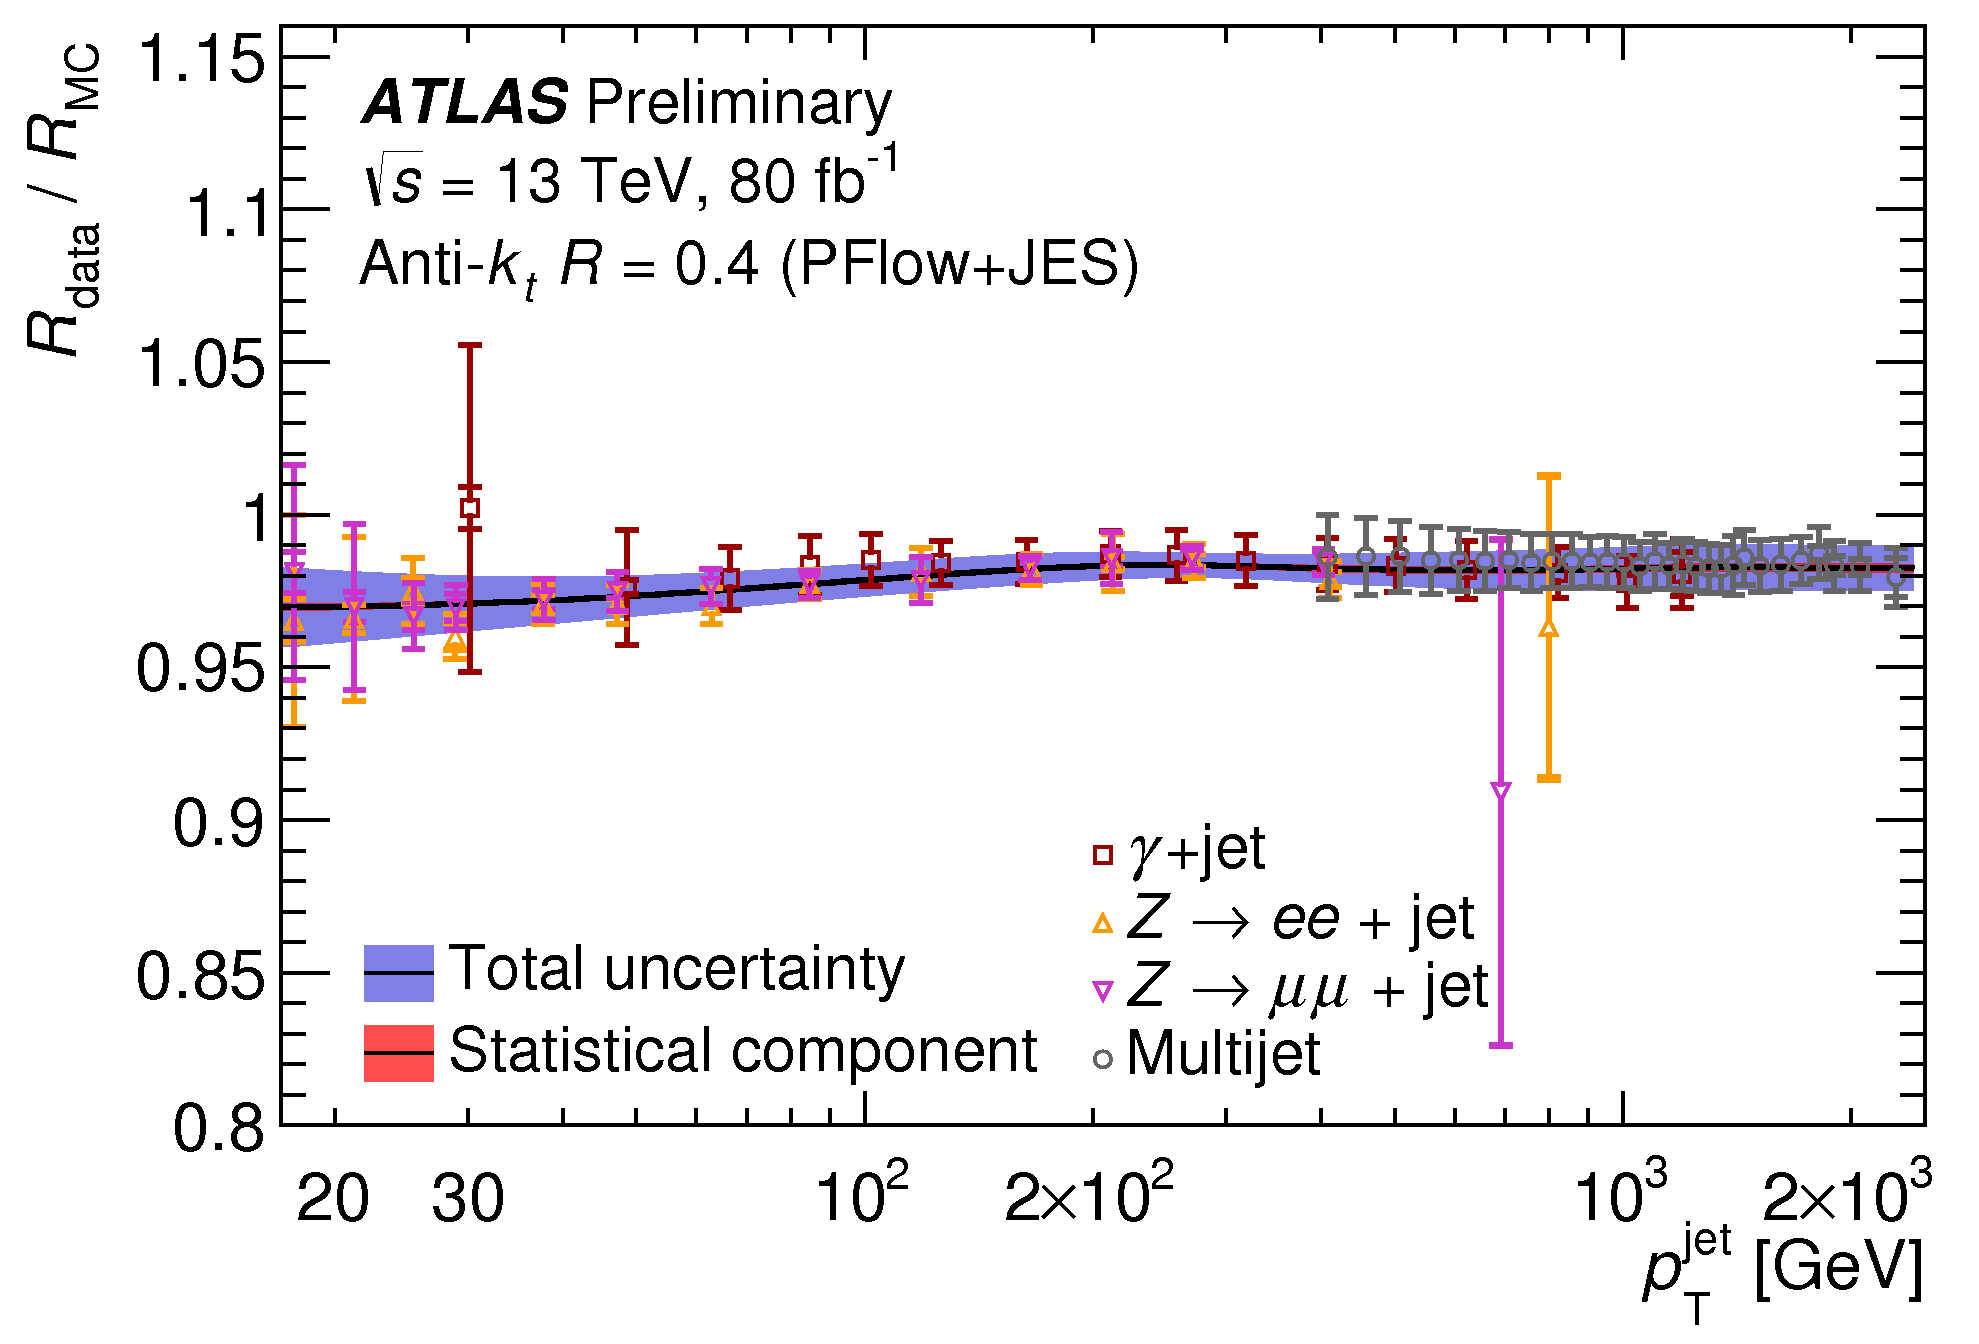
\includegraphics[width=\textwidth]{Pictures/ParticleFlowScale.png}
  \end{minipage}
  \hspace{.5cm}
  \begin{minipage}[b]{0.4\textwidth}
    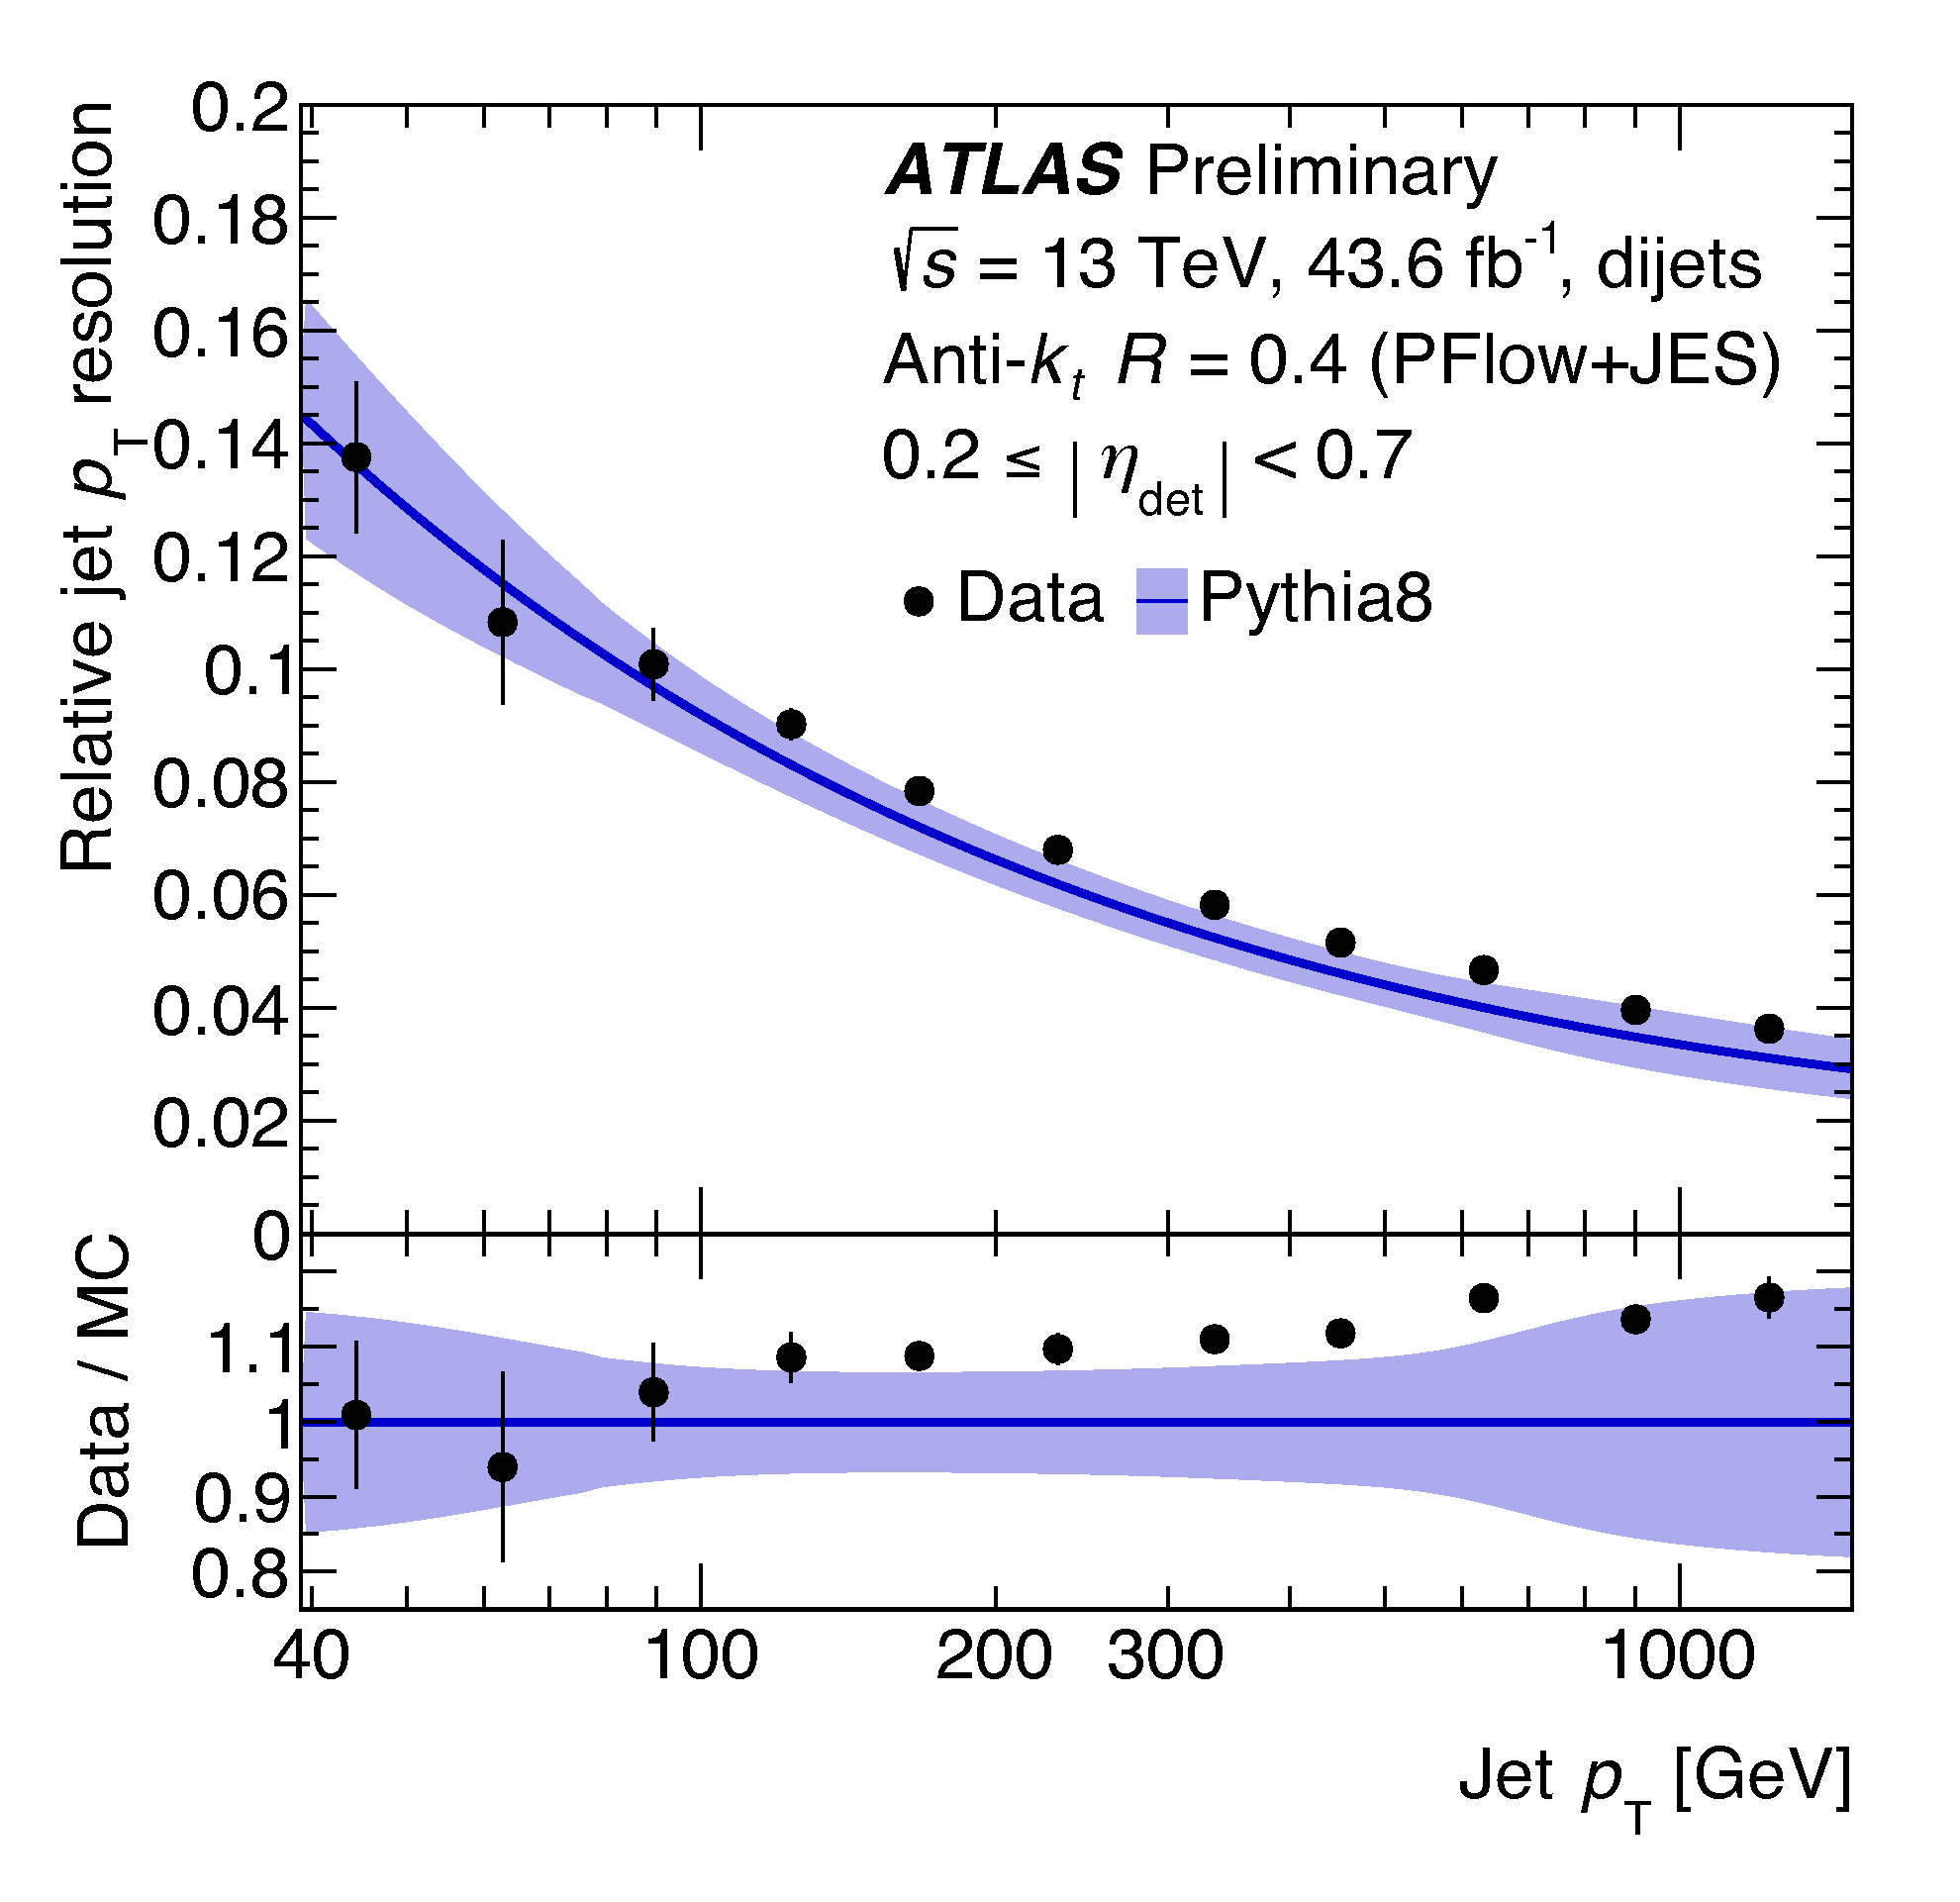
\includegraphics[width=\textwidth]{Pictures/ParticleFlowResolution.png}
  \end{minipage}
    \caption{ Left: data-to-simulation ratio for average jet $p_T$ as a function of jet $p_T$. Three techniques shown as well as their their combination (black) and the combination total uncertainty. PFlow Anti-$k_t$ jets with R=0.4 and JES correction. Right: relative jet energy resolution as a function of $p_T$ for anti-$k_t$ PFlow jets with $R=0.4$ in 2017. JES calibrations applied and compared to MC with full systematic uncertainties \cite{JETEtmiss}.}
    \label{fig:ScaleRes}
\end{figure}

Jet reconstruction and calibration are crucial to this analysis and later chapters will detail how impactful jet energy scale and resolution uncertainties are to the overall precision of the $H\rightarrow WW$ cross-section measurement. 

\section{Missing transverse energy}
Colliding protons in collider experiments like ATLAS have momentum solely in the plane of the beam. Conservation of momentum implies that in the plane transverse to the beam ($x-y$) the sum of momentum from all interaction by-products is zero. This is most often not the case and the non-zero transverse momentum from any interaction is termed $E_T^{miss}$. Missing transverse energy is a sign of final state neutrinos. $E_T^{miss}$ could also point to new particles that cannot be directly detected, like neutralinos or dark matter particles. $E_T^{miss}$ could also signify interacting particles which evade detection in ATLAS due to detector acceptance or poor reconstruction \cite{METSig}. 

Missing transverse energy is determined using a combination of all reconstructed particles in an event. This is challenging because it involves all detector components and final particle types. The Jet/$E_T^{miss}$ performance group delivers calibrations for multiple $E_T^{miss}$ variables that we use in the $H\rightarrow WW$. This section will discuss $E_T^{miss}$ reconstruction and performance followed by definitions of a few additional $E_T^{miss}$ observables. 
Reconstructed $E_T^{miss}$ calculations take into account both \textit{hard} and \textit{soft} event signals. Hard-events are composed of fully reconstructed and calibrated particles like electrons, muons, photons, $\tau$-leptons and jets. All other objects are considered \textit{soft}. Reconstruction for all particle types happens independently, which means that the same signal may be used to identify two distinct particles. This double-counting is taken into account in $E_T^{miss}$ resolution. At its most basic, $E_T^{miss}$ is defined:
\begin{equation}
E_{x(y)}^{miss}=-\sum_{i\in{\textnormal{hard objects}}}p_{x(y),i} -\sum_{j\in{\textnormal{soft objects}}}p_{x(y),j}
\end{equation}
where overall $E_T^{miss}$ is a vector composed of $x,y$ components. In order to avoid double-counting the same detector signal in multiple particle reconstruction algorithms, hard objects are consider in order: electrons, photons, hadronically decaying $\tau$-leptons, and then jets. Muons have little overlap since they are reconstructed using MS and ID tracks (and muons alone leave tracks in the MS). As particles are reconstructed in this sequence, signals used more than once are rejected to avoid overlap. Another key variable is $\sum E_T$ which is defined
\begin{equation}
\sum E_T = \sum_{\text{electrons}} p_T^e + \sum_{\text{photons}} p_T^\gamma + \sum_{\text{$\tau$-leptons}} p_T^\tau + \sum_{\text{muons}} p_T^\mu + \sum_{\text{jets}} p_T^{jet} - \sum_{\text{unused tracks}} p_T^{track}
\end{equation}
The first five terms show the hard term while the last represents the soft-term. Selections are applied to reconstructed jets and particles to achieve optimal $E_T^{miss}$ for a particular analysis \cite{METPerf}. In the context of $H\rightarrow WW$ we use a ``tight" configuration for $E_T^{miss}$ classified by strict conditions on accepted jets. This working point has the greatest pile-up rejection which is integral to our analysis. 

$E_T^{miss}$ reconstruction contains the complexity of each of its component parts and their $p_T$ resolutions all affect total $E_T^{miss}$ resolution. Pile-up and total event activity also play a large role in $E_T^{miss}$ performance. Validations for $E_T^{miss}$ are performed on a variety of observables and MC modelling is compared to reconstructed data. Systematic uncertainties are derived from comparing the reproducibility of these observables and their successful modelling of data. Resolution for reconstructed jets and leptons are also propagated to overall $E_T^{miss}$ uncertainty. $E_T^{miss}$ performance is evaluated using $Z\rightarrow \mu\mu$, $Z\rightarrow e^-e^+$, and $W\rightarrow e\nu$ events, the first two with no genuine $E_T^{miss}$ and the third with significant $E_T^{miss}$ from neutrinos. After specific event selection and $E_T^{miss}$ reconstruction, $E_T^{miss}$ for each of these samples is studied and data and MC are demonstrated to match within uncertainties. Selected performance observables are shown for the full Run-2 dataset in \ref{fig:METPerf}. Here $Z\rightarrow e^+e^-$ reconstructed track-based soft term $E_T^{miss}$ and $E_T^{miss}$ significance distributions are shown. Data and MC show good agreement.

\begin{figure}[!h]
    \centering
  \begin{minipage}[b]{0.45\textwidth}
  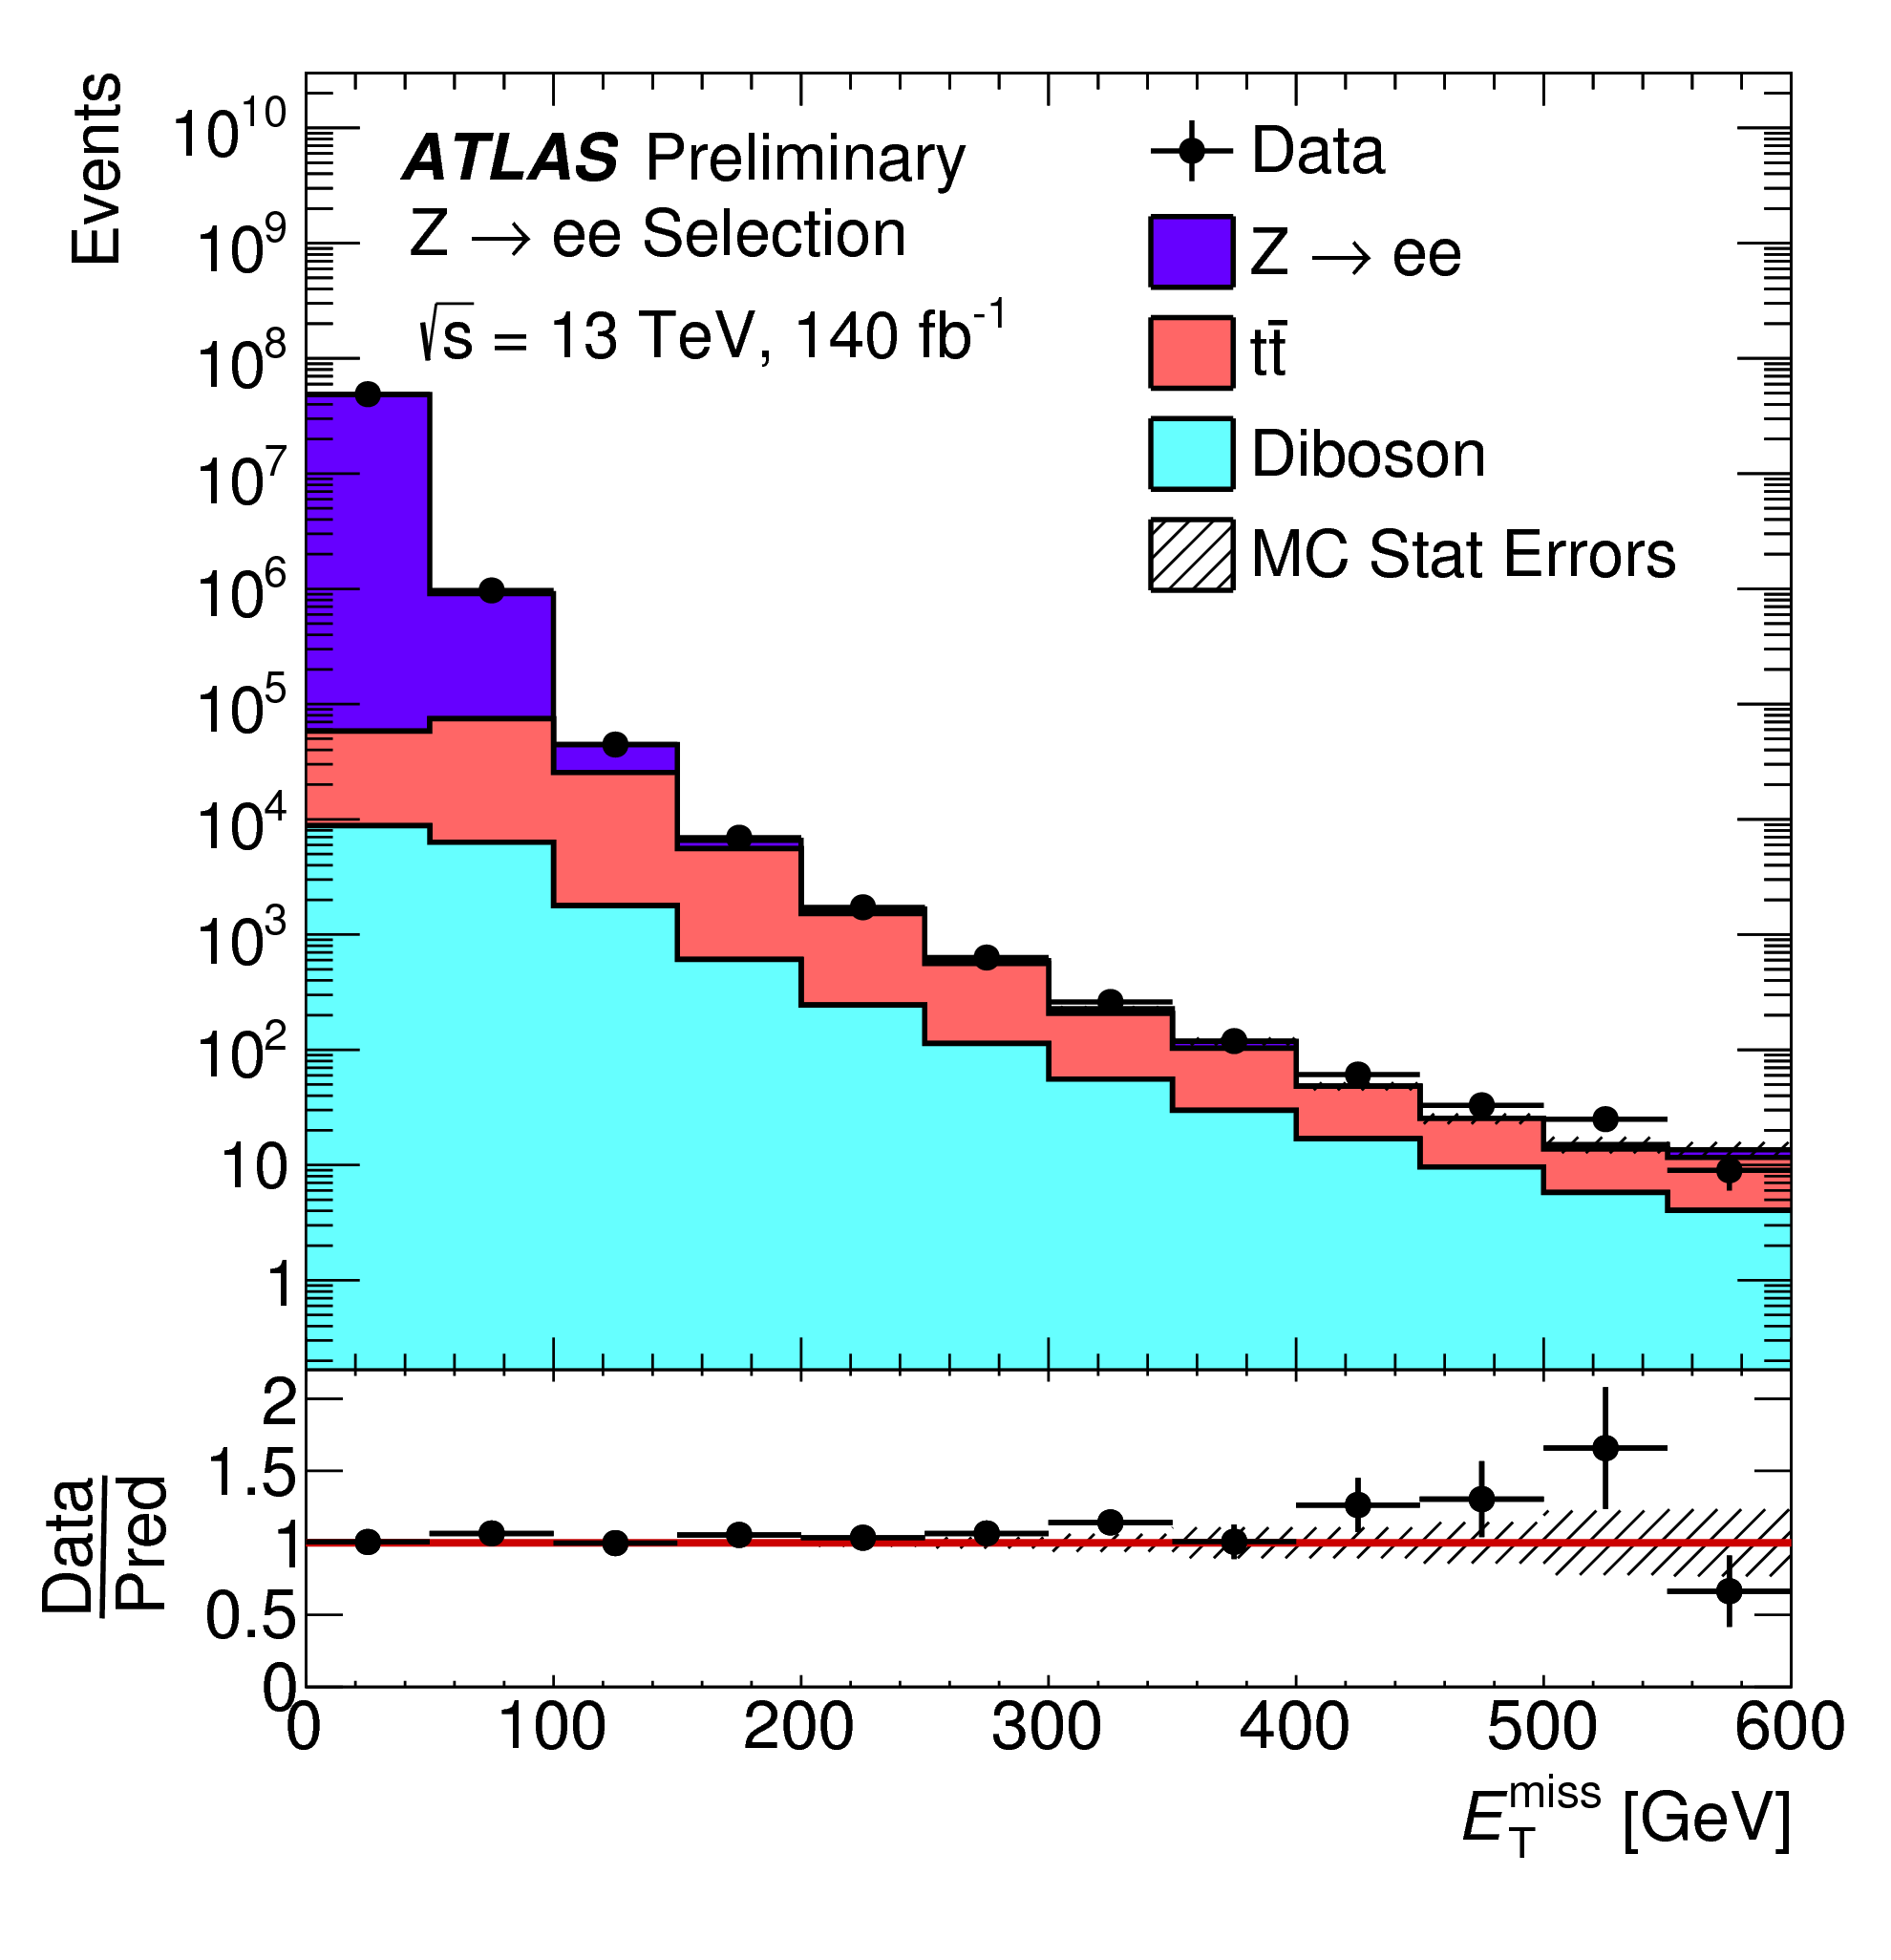
\includegraphics[width=\textwidth]{Pictures/ETMissPerf.png}
  \end{minipage}
  \hspace{.5cm}
  \begin{minipage}[b]{0.45\textwidth}
    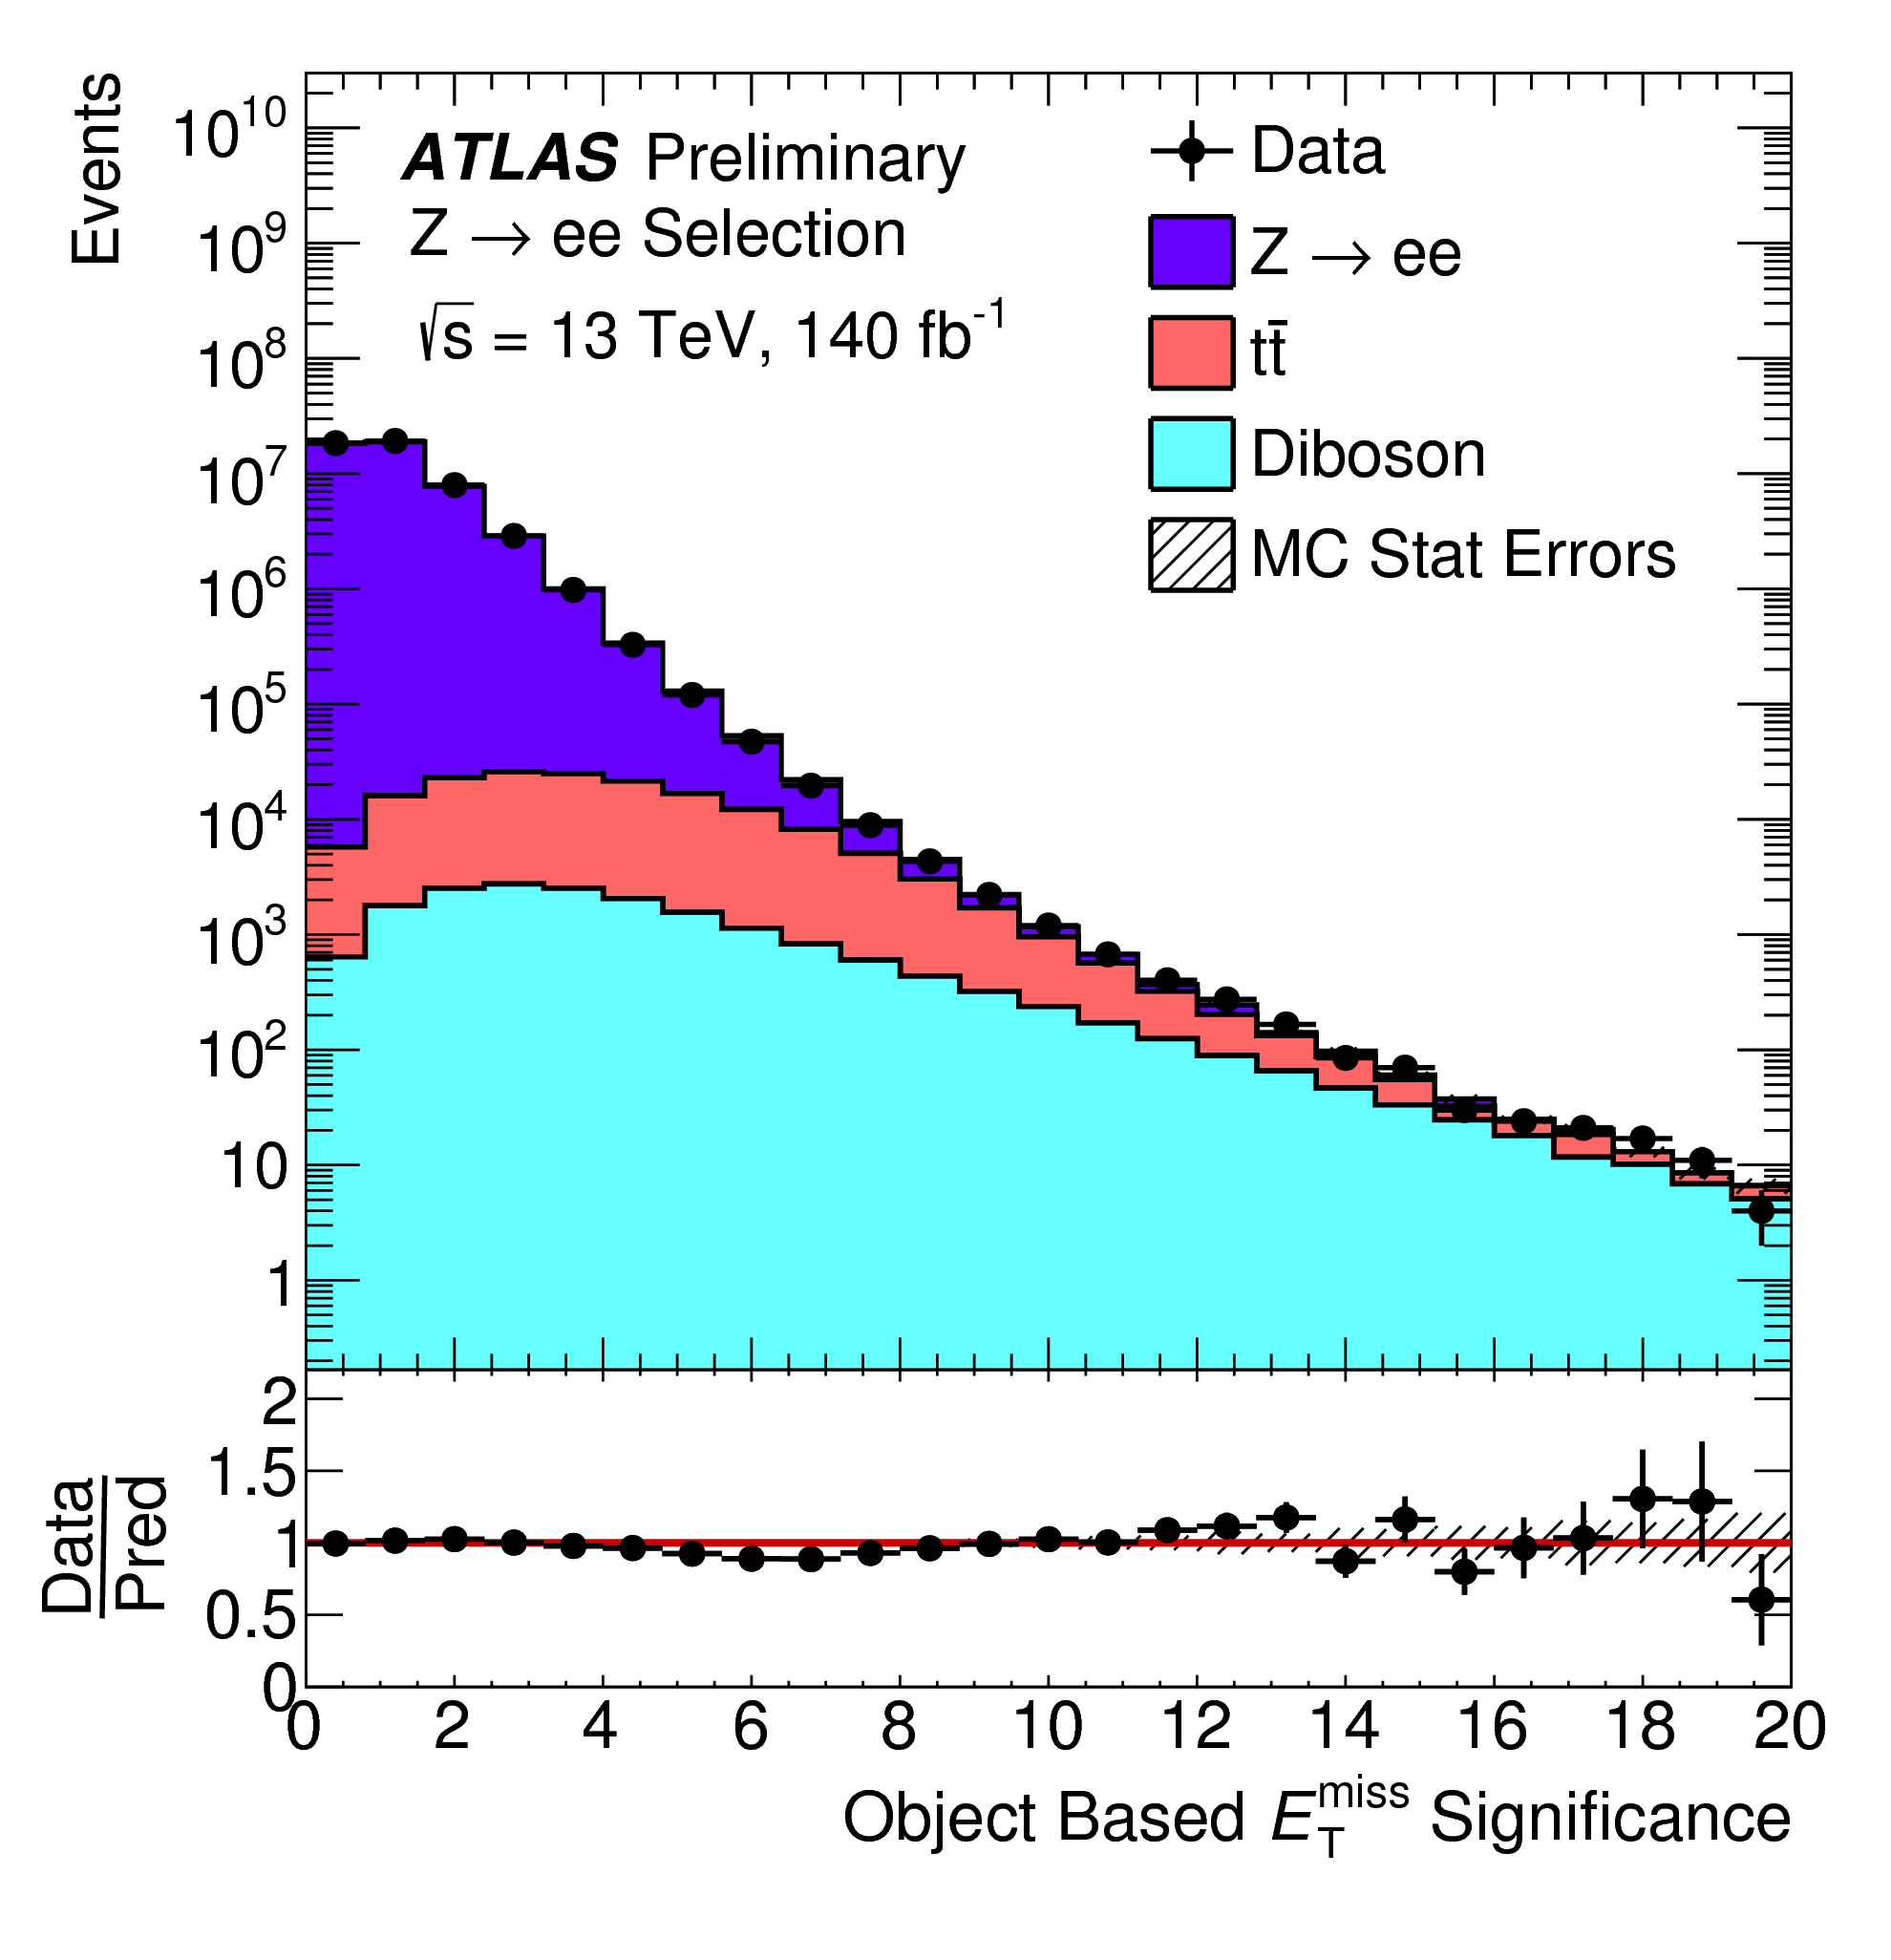
\includegraphics[width=\textwidth]{Pictures/ETMissSig.png}
  \end{minipage}
    \caption{ Left: Track-based Soft Term $E_T^{miss}$ shown for the complete Run-2 dataset with an integrated luminosity of 140 fb$^-1$. Monte Carlo simulations are compared to data for the tight $E_T^{miss}$ working point. Right: Track-based Soft Term $E_T^{miss}$ significance modelling shown in the tight $E_T^{miss}$ working point  \cite{JETEtmiss}}
    \label{fig:METPerf}
\end{figure}

In this analysis, a number of $E_T^{miss}$ variables are used. These variables are used to reject backgrounds particularly from $Z\rightarrow \tau\tau$ events, from signal, $H\rightarrow WW\rightarrow \ell\nu\ell\nu$, where its two neutrinos generate significant $E_T^{miss}$. Some of the variables used for these selections include track-based $E_T^{miss}$, track-based soft term $E_T^{miss}$, $m_{\tau\tau}$, $E_T^{miss}$ significance and $p_T^{tot}$. The $E_T^{miss}$ soft term is composed of a track-based and calo-based component. The calorimeter-based component is highly dependent on pile-up and so using a track-based soft term reduces overall pile-up dependence. Track-based $E_T^{miss}$ uses only reconstructed ID tracks from the primary vertex and in our analysis this has been just as powerful discriminant for isolating $Z\rightarrow \tau\tau$ background events from VBF signal as overall $E_T^{miss}$ without the same pile-up dependence and correlation with other kinematic variables. $E_T^{miss}$ significance is a newly defined and recommended variable from the Jet/$E_T^{miss}$group. Described further in \cite{METSig}, it discriminates real missing energy from momentum resolution effects using a calculated likelihood. Shown in \ref{fig:METPerf},  $E_T^{miss}$ significance peaks at low values if $E_T^{miss}$ likely comes from resolution effects and not from a real invisible particle in the event. Our analysis defines two additional variables based on $E_T^{miss}$: $p_T^{tot}$ describes the total transverse momentum from all hard objects in the event, and $m_{\tau\tau}$, defined as
\begin{equation}
m_{\tau\tau} = \frac{m_{\ell\ell}}{\sqrt{x_1*x_2}},
\end{equation}
where 
\begin{equation}
\begin{split}
x_1 = \frac{p^{\ell0}_x*p^{\ell1}_y-p^{\ell0}_y*p^{\ell1}_x}{p^{\ell1}_y*E_{Tx}^{miss}-p^{\ell1}_x*E_{Ty}^{miss}+p^{\ell0}_x*p^{\ell1}_y-p^{\ell0}_y*p^{\ell1}_x}, \text{and} \\
x_2 = \frac{p^{\ell0}_x*p^{\ell1}_y-p^{\ell0}_y*p^{\ell1}_x}{p^{\ell1}_x*E_{Ty}^{miss}-p^{\ell0}_y*E_{Tx}^{miss}+p^{\ell0}_x*p^{\ell1}_y-p^{\ell0}_y*p^{\ell1}_x}
\end{split}
\end{equation}
Each of these variables contributes to our signal region selection and elimination of background. A number of systematic uncertainties from reconstructed $E_T^{miss}$ are defined and used in our analysis, though these are small compared to the uncertainties from jets and other final state particles.

In this chapter, I have outlined the procedures for building all the physics objects we use in the $H\rightarrow WW$ analysis. The next chapters will use these physics objects and their kinematic variables to understand our background and signal events.
 
